\documentclass[12pt,a4paper,oneside,openright,titlepage,italian]{book}

\usepackage[italian]{babel}
\usepackage[latin1]{inputenc}
\usepackage{graphicx}
\usepackage{amsmath} 
\usepackage{amssymb}
\usepackage{longtable}
\usepackage{fancyhdr}
\usepackage{frontesp}
\usepackage{listings}
%\usepackage{fullpage}

%%\renewcommand{\thesection}{\arabic{section}}
\addtolength{\voffset}{-0,5cm}
\addtolength{\textheight}{1cm}
\setlength{\parindent}{0pt}
\frenchspacing
\linespread{2.0}

\pagestyle{fancy}
\renewcommand{\chaptermark}[1]{\markboth{#1}{}}
\renewcommand{\sectionmark}[1]{\markright{\thechapter .\thesection\ #1}}
\renewcommand{\subsectionmark}[1]{\markright{\thechapter .\thesubsection\ #1}}
\newcommand\Item[1]{\emph{(#1)}}
\newcommand\celsius{\,^{\circ}\mathrm{C}}
\fancyhf{}
\lhead{\rightmark}
\chead{}
\rhead{\bfseries\thepage}
\renewcommand{\headrulewidth}{0.4pt}
\renewcommand{\footrulewidth}{0pt}
%\setlength{\headheight}{15pt}
\setlength{\headheight}{40pt}
\fancypagestyle{plain}{\fancyhead{}\renewcommand{\headrulewidth}{0pt}}
\fancyhead[RO]{\textbf{\thepage}}
\fancyhead[LO]{\nouppercase{\rightmark}}


\begin{document}
%\addtolength{\oddsidemargin}{+1,3cm}
\addtocounter{tocdepth}{+1}

\begin{titlepage}
\begin{center}
  {\Large \sc Universit\`a degli Studi di Catania}\\
  {\large \sc Facolt\`a di Ingegneria}\\
  {\sc Corso di Laurea Specialistica in Ingegneria Informatica}\\
  %{\sc Dipartimento di Ingegneria Informatica e delle Telecomunicazioni}\\
  
  \hbox to \textwidth{\hrulefill}
  
  \vspace{1.8truecm}
  
  {\large \sc Loris Fichera}
  
  \vspace{1.8truecm}
  
  {\large\sc \uppercase{\textbf{De Bello Gallico}}} %%\\
  %%{ {\sc Sottotitolo}}
  
  \vspace{1.7truecm}
  
  %\centerline{\hbox to 3.5truecm{\hrulefill}}
  \begin{tabular}{c}
    \hline
        {\sc Tesi di Laurea}\\
        \hline
  \end{tabular}
  %\centerline{\hbox to 3.5truecm{\hrulefill}}

  \vspace{1.7truecm}
  
  \begin{minipage}{\textwidth}
    \begin{flushright}
      \begin{minipage}{0.3\textwidth}
        \begin{tabbing}
          Relat\=ore:\\
          \>  \=Chiar.mo Prof. \= {\sc C. Santoro}
        \end{tabbing}
      \end{minipage}
    \end{flushright}
  \end{minipage}
  
  %\vspace{1truecm}
  
  \hbox to \textwidth{\hrulefill}
        {\sc Anno Accademico 2010/2011}        
\end{center}
\end{titlepage}

\endinput


%% \dedica {The last good thing written in C was Franz Schubert's Symphony number 9.\\
%%   \emph{Erwin Dieterich}}


\dedica {
  The world is concurrent.\\
  Things in the world don't share data.\\
  Things communicate with messages.\\
  Things fail.\\
  \emph{Joe Armstrong}
}

\begin{small}
\makededica
\end{small}
\tableofcontents
\listoffigures
\lstlistoflistings
\newpage

\clearpage{\pagestyle{empty}\cleardoublepage}
\chapter*{Introduzione} 
%%\markboth{Introduzione}{Introduzione}
\addcontentsline{toc}{chapter}{Introduzione}
%

%
Secondo il rapporto sullo stato del solare fotovoltaico in Italia
\cite{gse2010}, pubblicato dal \emph{Gestore dei Servizi Energetici}
(GSE) nell'Aprile del 2011, il numero di impianti fotovoltaici
presenti sul territorio nazionale al 31 dicembre 2010 \`e pari 
a 155977, per una potenza nominale complessiva di circa 3469,9 MW.
%
Tali valori si inseriscono all'interno di un trend di crescita, 
mostrato in figura \ref{fotovoltaico-italia}, decisamente sostenuto: 
solo nel 2010, il numero di impianti \`e raddoppiato, mentre la potenza 
nominale \`e addirittura triplicata.
%
Tra le motivazioni alla base di tale crescita, vi \`e sicuramente il 
programma di incentivazione, noto come \emph{Conto Energia}\cite{camera2003},
riservato ai soggetti responsabili di impianti fotovoltaici.
%% %
\begin{figure}[!h]
\centering
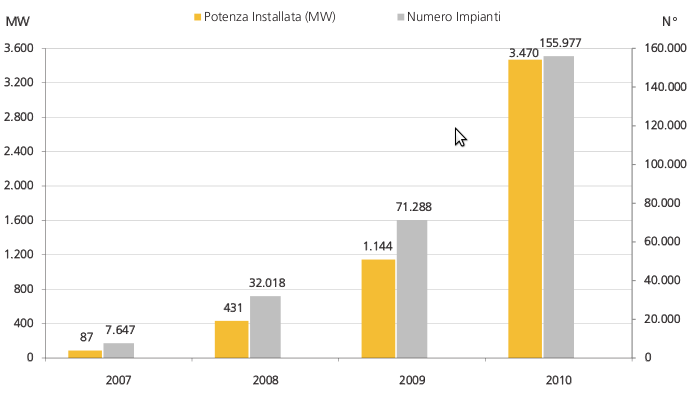
\includegraphics[width=350pt]{img/trend-fotovoltaico-italia.png}
\caption{Trend di crescita del fotovoltaico in Italia}
\label{fotovoltaico-italia}
\end{figure}
%% %
%
\`E interessante osservare che oltre il 90\% degli impianti installati
appartiene alla classe di potenza medio-bassa, i.e. la potenza nominale
non supera i 20kW. 
%
Ci\`o rende l'idea di come la produzione di energia
elettrica mediante fotovoltaico sia fortemente \emph{distribuita} 
sul territorio, in contrasto con i metodi di produzione mediante 
fonti \emph{convenzionali}, ad esempio carbone e gas, che avviene 
in pochi grandi impianti, ciascuno in grado di sviluppare potenze molto 
elevate.
%

%
In un contesto caratterizzato da una crescita vertiginosa e da una 
elevata frammentazione geografica degli impianti, il problema del
\emph{monitoraggio}, inteso come verifica \emph{continuativa} e \emph{remota}
dello stato di un impianto, %% !FIXME che brutta espressione
assume una grande rilevanza: il soggetto responsabile della manutenzione
dell'impianto necessita di uno strumento che gli permetta di
effettuare diagnosi di eventuali malfunzionamenti \emph{da remoto}, cio\'e 
senza intervenire fisicamente sull'impianto; d'altro canto, il soggetto 
responsabile dell'impianto, ovvero il proprietario, \`e interessato 
a verificare se e quanto l'impianto sta producendo, e, quindi, 
tenere sotto controllo il ritorno sull'investimento effettuato.

%% descrizione del contenuto della tesi

\clearpage{\pagestyle{empty}\cleardoublepage}
\chapter{Introduzione al fotovoltaico}
%
Per \emph{impianto fovoltaico} si intende un qualunque 
impianto di produzione di energia elettrica che sfrutti, ai fini 
di produzione della stessa, l'\emph{effetto fotovoltaico}.
%
Ne esistono due grandi tipologie: impianti \emph{a isola} (o \emph{stand alone}), 
e impianti \emph{grid connected}, ovvero connessi alla rete nazionale in 
corrente alternata.
%
Oggetto di questa tesi saranno solo questi ultimi, in quanto sono gli unici
di cui abbia senso monitorare e quantificare la produzione energetica; gli impianti 
a isola, infatti, non sono generalmente utilizzati per la produzione di grandi
quantit\`a d'energia, piuttosto trovano applicazione laddove \`e necessario
rendere un sistema elettricamente \emph{autosufficiente}, p.es. per la 
ricarica di dispositivi alimentati a batteria.
%

%
Iniziamo la panoramica sugli impianti fotovoltaici partendo dal fenomeno
che sta alla base del loro funzionamento: l'effetto fotovoltaico.
%

%
\section{L'effetto fotovoltaico}
L'\emph{effetto fotovoltaico} consiste nel passaggio di elettroni 
dalla \emph{banda di valenza} alla \emph{banda di conduzione} di 
un materiale, a causa dell'assorbimento di \emph{fotoni}. 
%
Tale fenomeno viene sfruttato dai \emph{moduli (o celle) fotovoltaici}, 
come mostrato in figura \ref{effetto-fv} allo scopo di trasformare 
l'energia insita nella radiazione luminosa in energia elettrica.
%
\begin{figure}[!h]
\centering
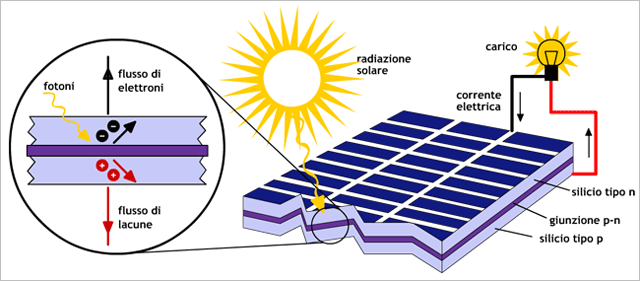
\includegraphics[width=350pt]{img/effetto-fovoltaico.png}
\caption{Effetto fotovoltaico}
\label{effetto-fv}
\end{figure}
%

%
\section{Architettura degli impianti grid-connected}
Gli impianti fotovoltaici grid connected, detti anche \emph{campi fotovoltaici}, 
sono costituiti da un insieme di dispositivi \emph{in cascata}, come mostrato in 
figura \ref{impiantogridconnect}: \emph{a monte} di tutto si trovano i \emph{moduli 
fotovoltaici}, ovvero i dispositivi che, sfruttando l'effetto fotovoltaico, 
producono energia elettrica. \emph{A valle} di questi, troviamo gli \emph{inverter}, 
macchinari il cui compito \`e quello di trasformare l'energia prodotta dai moduli 
in una forma tale che possa essere ceduta alla rete di distribuzione. Infine, tra 
gli inverter e la rete, il GSE provvede all'installazione di un \emph{contatore 
bidirezionale}, il cui scopo \`e quello di quantificare la produzione dell'impianto.
%% un impianto si caratterizza per la quantita` di energia di picco
\begin{figure}[!h]
\centering
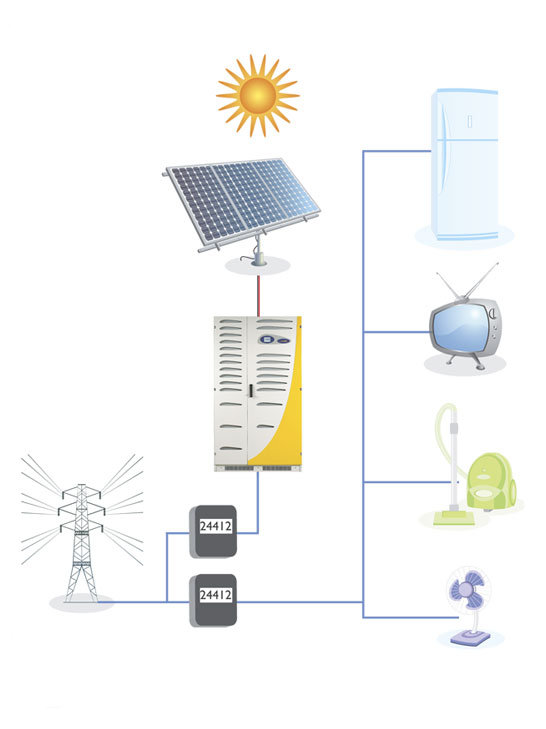
\includegraphics[width=350pt]{img/impianto-grid-connect.jpg}
\caption{Schema di impianto grid-connected con scambio sul posto}
\label{impiantogridconnect}
\end{figure}
%

%
Come gi\`a anticipato, gli impianti grid-connected immettono direttamente in rete 
l'energia prodotta. Per questo tipo di impianti, il GSE prevede uno schema di compensazione 
noto come \emph{scambio sul posto}\cite{scambioposto}, secondo cui l'energia immessa 
in rete pu\`o essere prelevata successivamente per i propri consumi.
%

%
\subsection{I moduli fotovoltaici}
I moduli fotovoltaici sono gli elementi produttivi di un impianto. 
Si tratta di dispositivi costituiti da \emph{celle} di materiale 
\emph{semiconduttore}, caratterizzato quindi da un \emph{band gap} 
di dimensioni tali per cui 
%
\begin{itemize}
\item a seguito dell'apporto energetico fornito dalla radiazione luminosa, 
      gli elettroni riescono a \emph{saltare} dalla banda di valenza a 
      quella di conduzione\footnote{ci\`o non sarebbe possibile in un \emph{isolante}}
%
\item gli elettroni che effettuano il \emph{salto} nella banda di conduzione 
      non vengono neutralizzati
      \footnote{come, invece, avverrebbe in un \emph{conduttore}}
\end{itemize}
%
La presenza di \emph{portatori di carica} nella banda di conduzione 
fa si che il modulo fotovoltaico, una volta connesso ad un conduttore 
esterno, si comporti come un \emph{generatore di corrente}\cite{bellini09}.
%
\begin{figure}[!h]
\centering
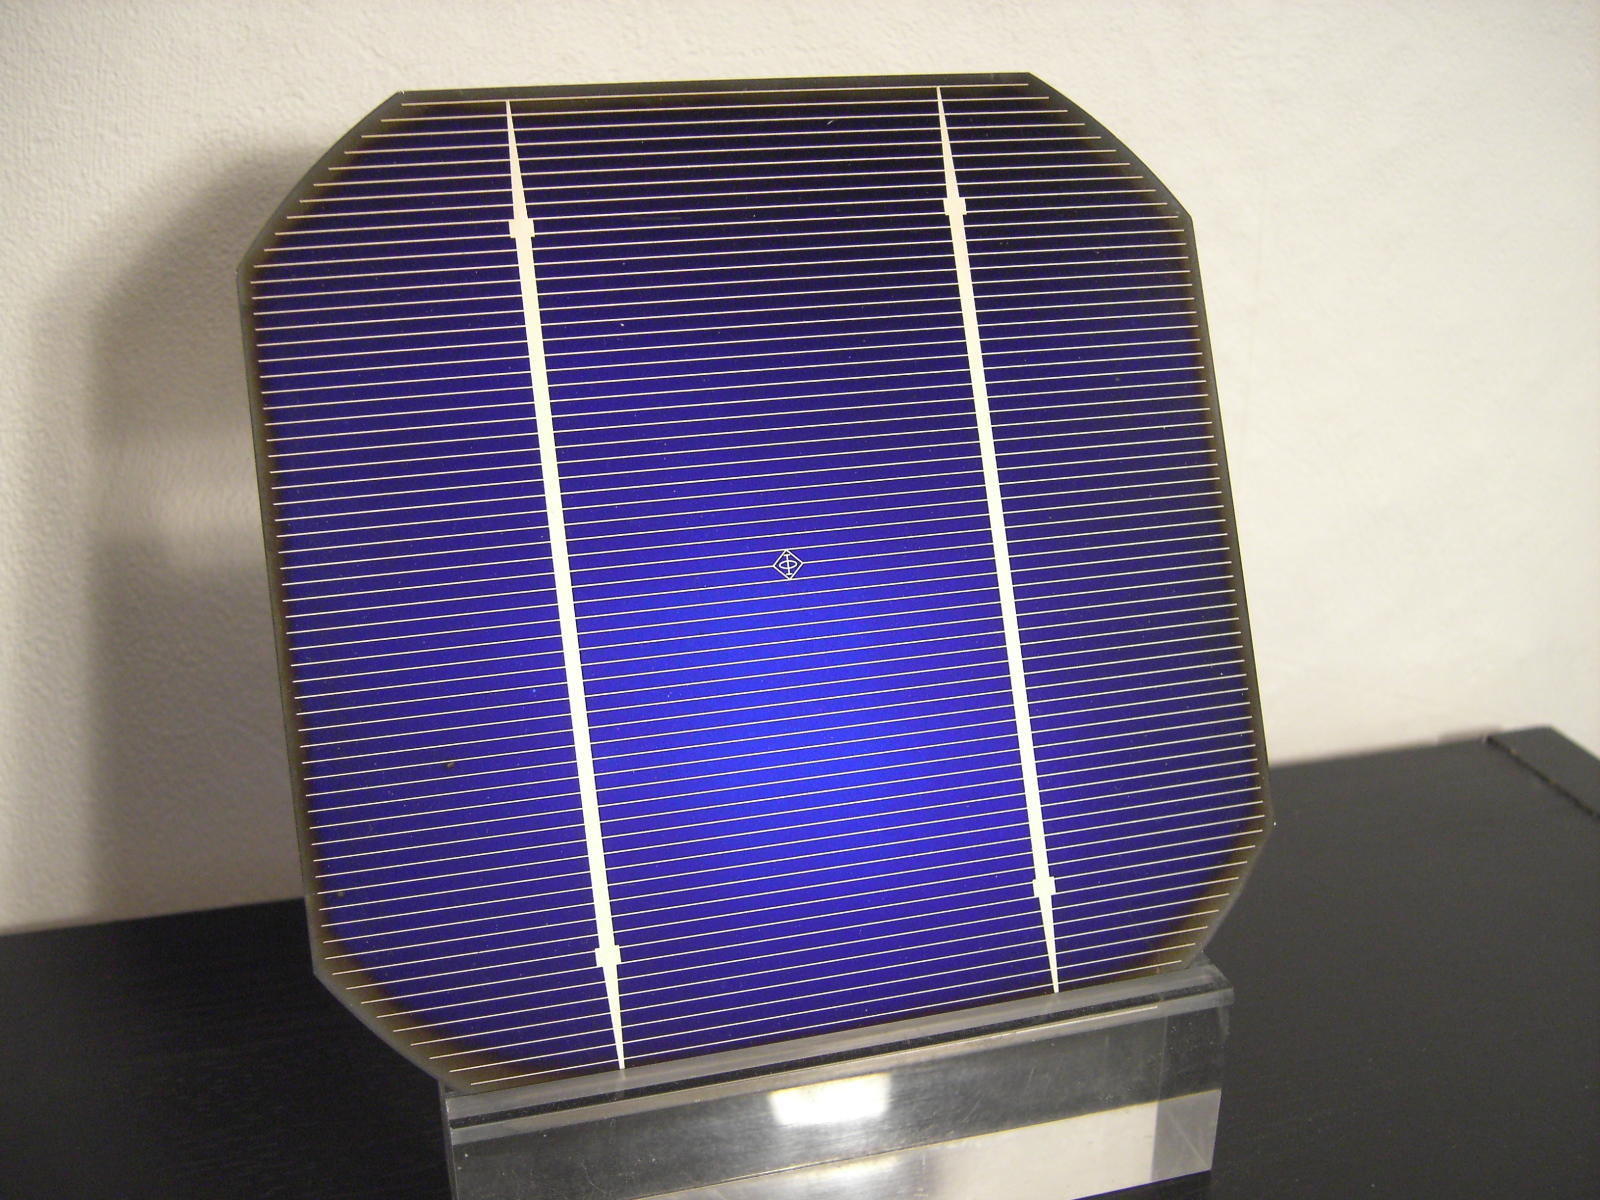
\includegraphics[width=350pt]{img/modulo-fotovoltaico.jpg}
\caption{Modulo fotovoltaico in silicio \emph{monocristallino}}
\end{figure}
%
Allo stato attuale, esistono diverse tecnologie di realizzazione di 
moduli fotovoltaici, la maggior parte delle quali basate su processi 
al silicio.
%

%
Per ogni modello di modulo fotovoltaico, le aziende 
costruttrici forniscono un \emph{datasheet}, riportanti i 
\emph{dati di targa} del modulo.
%
Tra i dati di targa, particolare importanza rivestono le curve 
\emph{corrente-tensione}, le quali caratterizzano l'andamento della tensione 
e della corrente - e, quindi, della potenza generata - ai capi del modulo, al 
variare di determinate \emph{grandezze d'influenza}.
%
Le curve corrente-tensione vengono tipicamente costruite mediante misurazioni
effettuate sotto \emph{standard test conditions} (STC)\cite{testconditions}, 
come indicato in tabella \ref{stc}, e variando di volta in volta una delle 
grandezze di influenza.
%
\begin{table}[htpb]
 \begin{center}
  \begin{tabular}{ | l | l | }
    \hline
    Radiazione & 1000 $W/m^2$ \\
    \hline
    Temperatura del modulo & 25  $\celsius$ \\
    \hline 
    Vento & 0 $m/s$ \\
    \hline
  \end{tabular}
  \caption{Condizioni di test standard (STC)}
  \label{stc}
 \end{center}
\end{table}
%

%
Un tipico esempio di curve corrente-tensione \`e mostrato in figura 
\ref{caratteristica_modulo_fv}: il primo dei due grafici mostra l'andamento 
della caratteristica al variare della radiazione solare, il secondo
invece mostra cosa accade al variare della temperatura superficiale del modulo.
%
\begin{figure}[!h]
\centering
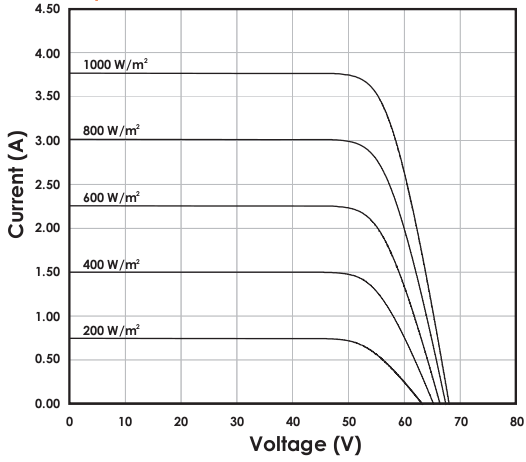
\includegraphics[width=190pt]{img/a-v-irradiance.png}
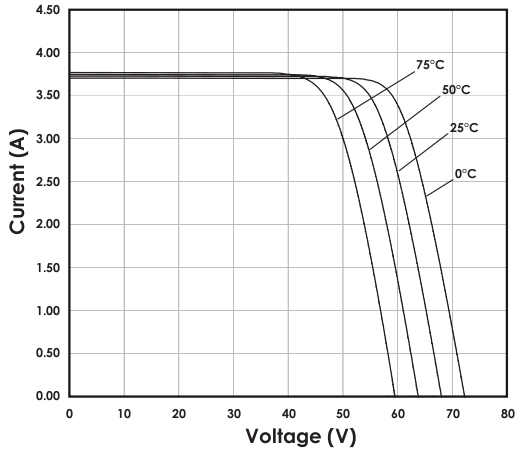
\includegraphics[width=190pt]{img/a-v-temperature.png}
\caption{Esempi di curve caratteristiche di un modulo fotovoltaico}
\label{caratteristica_modulo_fv}
\end{figure}
%% parlare della resistenza dei moduli e del decadimento delle prestazioni?
%% parlare dell'effetto dell'orientamento dei moduli rispetto alle prestazioni?
%

%
\subsection{Le stringhe fotovoltaiche}
Per \emph{stringa fotovoltaica} si intende un insieme di moduli connessi in \emph{serie}, 
come mostrato in figura \ref{stringa}.
%
La connessione in serie dei moduli \`e resa possibile da apposite \emph{junction box}, 
generalmente collocate sul retro dei moduli.
%

%
\begin{figure}[!h]
\centering
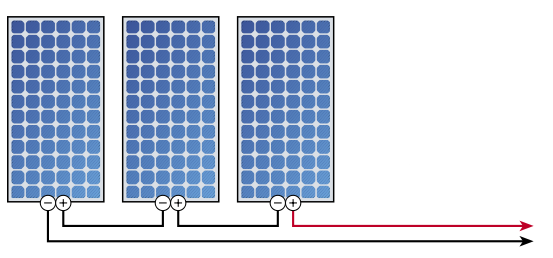
\includegraphics[width=350pt]{img/pv-string.png}
\caption{Connessione in serie di moduli fotovoltaici}
\label{stringa}
\end{figure}
%
%
\begin{figure}[!h]
\centering
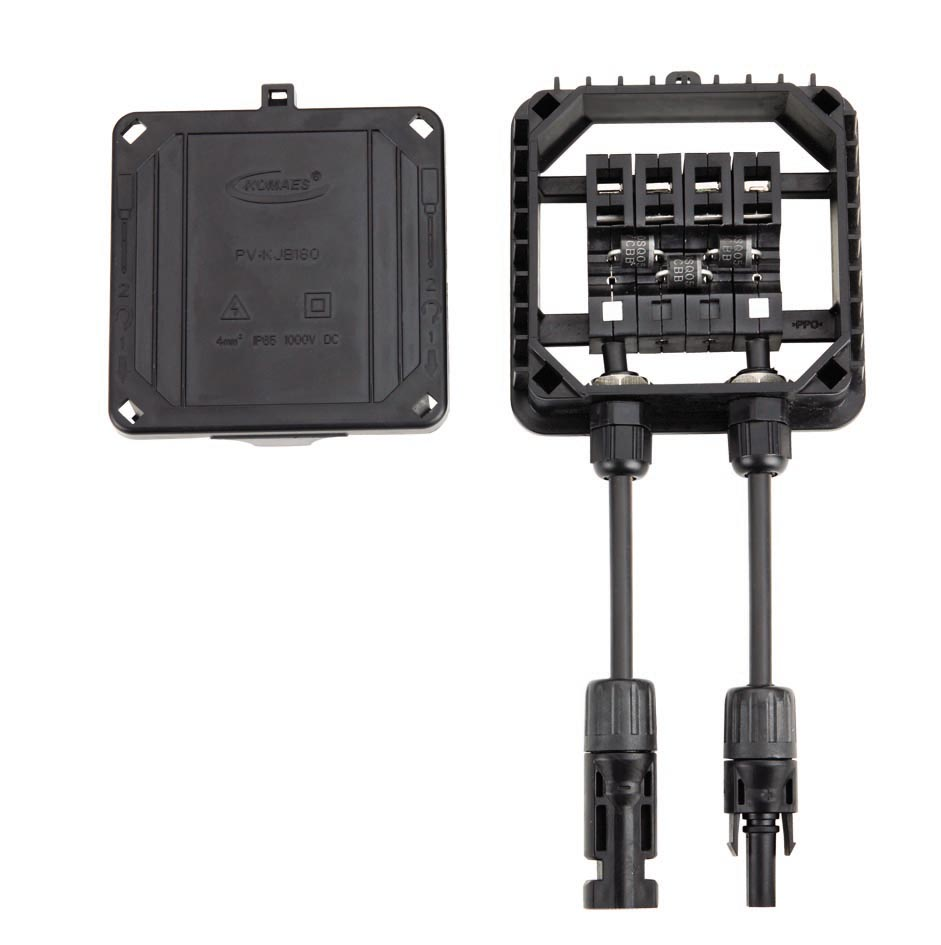
\includegraphics[width=180pt]{img/pv-junction-box.jpg}
\caption{Junction box}
\end{figure}
%

%
\`E importante evidenziare come connettere i moduli in serie condizioni le 
prestazioni dell'intera stringa: la legge di Ohm, infatti, impone che ogni 
modulo connesso in serie venga attraversato dalla stessa quantit\`a di corrente;
per cui, un degrado, anche temporaneo, delle prestazioni o, peggio, il 
malfunzionamento di uno dei moduli, provoca un peggioramento di produzione 
per tutti i moduli della stringa.
%
Tale fenomeno, noto come \emph{mismatch di corrente}, pu\`o manifestarsi,
ad esempio, nel caso in cui uno o pi\`u moduli siano, anche solo parzialmente, 
\emph{ombreggiati}, come mostrato in figura \ref{ombreggiamento}.
%
\begin{figure}[!h]
\centering
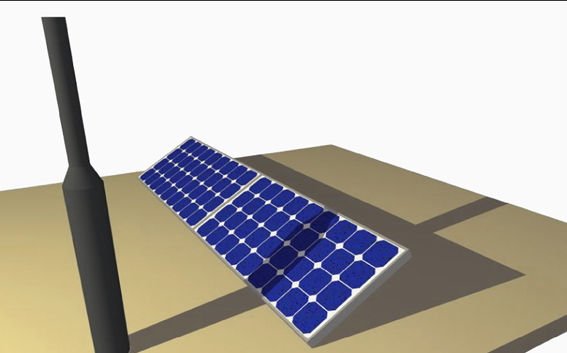
\includegraphics[width=300pt]{img/fv-ombreggiamento.png}
\caption{Ombreggiamento parziale di una stringa}
\label{ombreggiamento}
\end{figure}
%

%
Per limitare il manifestarsi di questo fenomeno, durante la fase di progettazione 
dei campi fotovoltaici vengono considerati fattori quali \Item{i} l'orientamento 
dei moduli della stringa, \Item{ii} la presenza di oggetti che possano produrre 
ombreggiamenti, \Item{iii} la distanza tra i moduli, \Item{iv} le caratteristiche 
climatiche della zona che ospiter\`a il campo fotovoltaico.
%

% dire che piu` stringhe possono essere collegate in parallelo
%
\subsection{Gli inverter}
La corrente continua prodotta dalle stringhe non pu\`o essere direttamente
immessa in rete. Si rendono necessari dei dispositivi, detti \emph{inverter}, 
in grado di trasformare la corrente continua in corrente alternata, alla 
stessa frequenza di quella della rete di distribuzione.
%

%
Nel contesto di un campo fotovoltaico, gli inverter sono quindi collocati a 
giunzione delle stringhe con la rete di distribuzione esterna. 
%
Come intuibile, si tratta dei componenti pi\`u complessi e critici degli 
impianti fotovoltaici: una loro avaria pu\`o compromettere il processo di 
distribuzione dell'energia prodotta dai moduli.
%

%
%
\begin{figure}[!h]
\centering
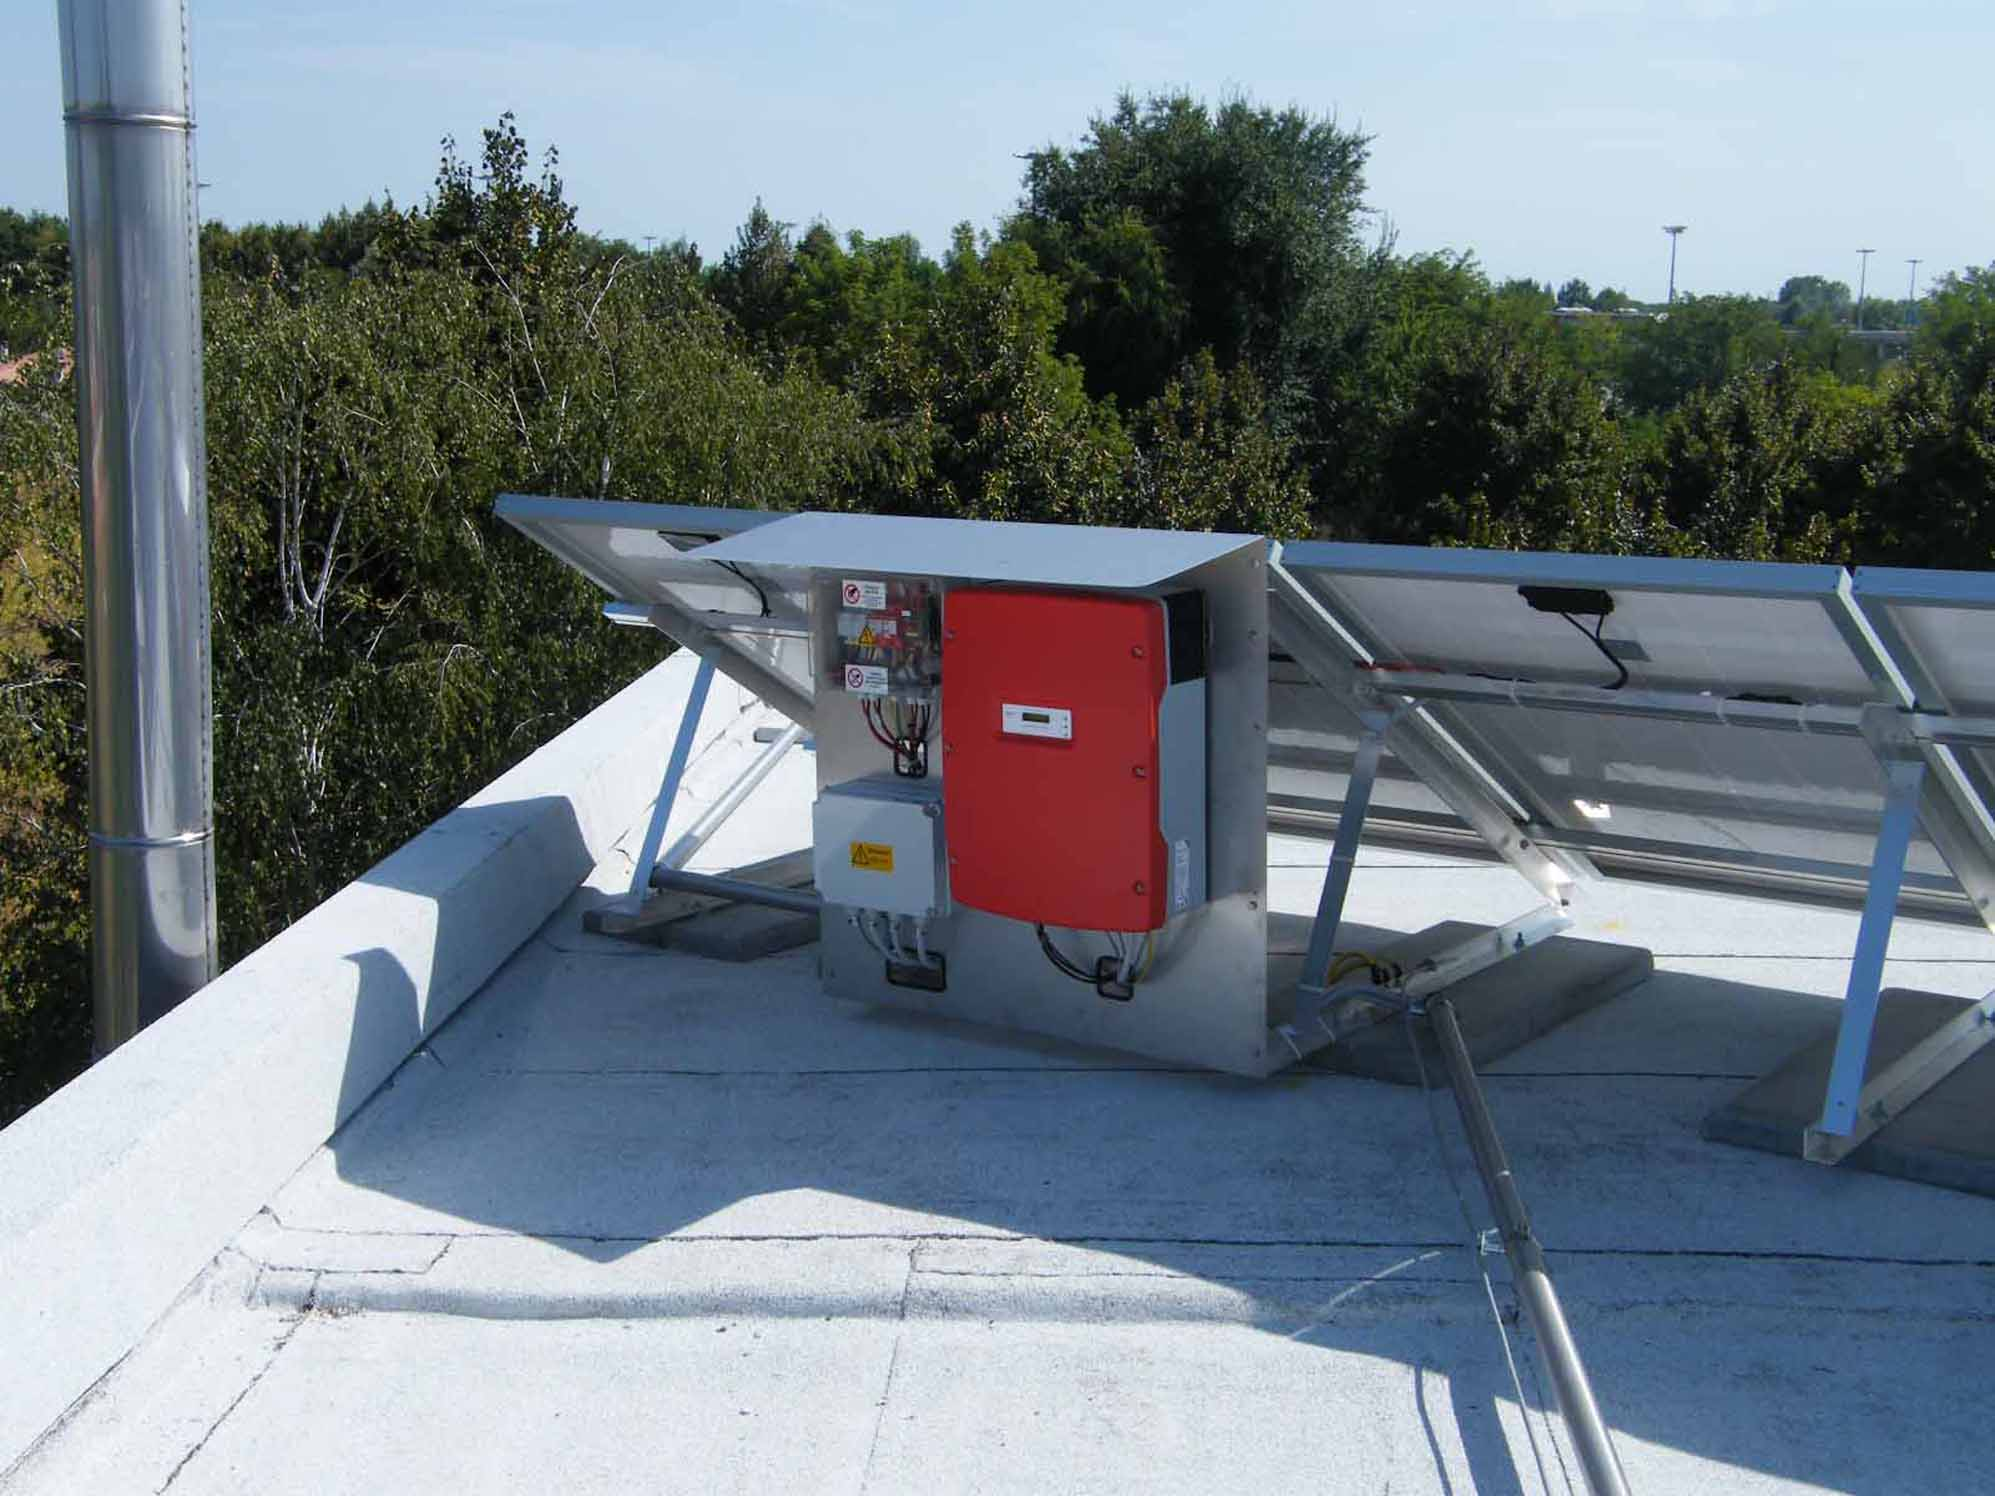
\includegraphics[width=300pt]{img/pv-inverter.jpg}
\caption{Inverter fotovoltaico}
%%\label{ombreggiamento}
\end{figure}
%
Tra i dati di targa di un inverter, particolare importanza riveste la sua 
\emph{efficienza}, definita come il rapporto tra l'energia in uscita 
(ceduta dall'inverter alla rete di distribuzione) e l'energia in ingresso 
(prodotta dalle stringhe).
%
Il valore di efficienza di un inveter non \`e determinato solo dalla 
non idealit\`a del processo di trasfomazione: parte dell'energia in ingresso, 
infatti, viene utilizzata dallo stesso inverter come alimentazione.
%
Gli inverter oggi presenti in commercio sono caratterizzati da valori tipici di
efficienza superiori al 95\%. Tuttavia, \`e da tenere in conto che l'efficienza 
di un inverter, a causa dell'effetto combinato di tempo e usura, tende a 
subire delle degradazioni.
%

%
Gli inverter progettati specificatamente per il fovoltaico presentano una gamma 
di funzionalit\`a che va oltre la sola trasformazione di corrente continua 
in alternata. Essi, infatti, sono spesso dotati di particolari sistemi di 
controllo, come il \emph{maximum power point tracker} (MPPT) che regolano la tensione 
di stringa in modo tale da estrarre dai moduli la massima potenza disponibile 
in qualsiasi condizione di irraggiamento.
%

%
Opzionalmente, gli inverter possono anche essere provvisti di un \emph{data logger}, 
i.e. un dispositivo che registra, nel tempo, i valori di grandezze di interesse quali 
correnti, tensioni, potenze ed energia prodotta.
% di notte gli inverter si spengono

%
\subsection{Il problema del rifasamento}
%
In regime di corrente alternata, la potenza elettrica $(S)$ \`e il risultato della 
somma di due componenti vettoriali: una \emph{attiva} $(P)$, traformabile in 
\emph{lavoro} e una \emph{reattiva} $(Q)$.
%
La presenza della componente reattiva \`e il diretto risultato dell'azione delle 
reattanze presenti in un circuito, i.e. induttori e/o condensatori, le quali 
provocano uno \emph{sfasamento} tra corrente e tensione, rappresentato in 
figura \ref{potenzaattivareattiva} dall'angolo $\varphi$.
%

%
\begin{figure}[!h]
\centering
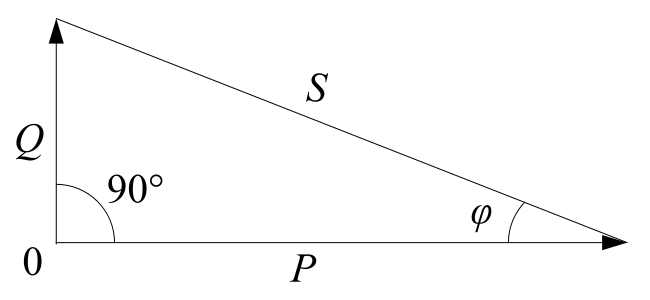
\includegraphics[width=250pt]{img/apparent-power.png}
\caption{Rappresentazione vettoriale di potenza attiva e reattiva}
\label{potenzaattivareattiva}
\end{figure}
%
Bench\'e si tratti di una componente inutilizzabile, la presenza della potenza 
reattiva va tenuta in considerazione nel dimensionamento dei sistemi di 
distribuzione. \`E per questo motivo che il gestore della rete elettrica in 
bassa tensione impone dei limiti circa le quantit\`a di potenza reattiva 
che le utenze sono autorizzate a scambiare con la rete stessa.
%

%
Per rispettare tali limiti, indicati in \cite{criteriallacciamento}, gli impianti 
fotovoltaici possono essere dotati di sistemi di \emph{rifasamento}, posti 
tra gli inverter e il contatore di scambio, il cui scopo \`e l'azzeramento 
dell'angolo $\varphi$.
%

%
\section{Il problema del monitoraggio}
Terminata la breve panoramica sugli impianti fotovoltaici, introduciamo il 
problema alla base del presente lavoro di tesi: il monitoraggio degli impianti 
fotovoltaici.
%

%
Il problema del monitoraggio pu\`o essere formulato mutuando concetti e 
terminologia dalla disciplina del \emph{controllo dei processi industriali}: 
la produzione di energia elettrica mediante moduli fotovoltaici pu\`o essere
modellata, infatti, come un \emph{processo continuo} caratterizzato dalle 
seguenti \emph{variabili di stato}:
%
\begin{itemize}

\end{itemize}



%% cosa monitorare: tensioni, correnti, potenze, energie
%% cosa monitorare: degradazione delle performance dei singoli componenti





%% architettura tipica di un impianto fotovoltaico
%% quali informazioni si vogliono produrre?
%% quali informazioni e` necessario rilevare?
%% lista dei desiderata per un sistema di monitoraggio
 %% definizione del problema
\clearpage{\pagestyle{empty}\cleardoublepage}
\chapter{Architettura del sistema}
%
Il sistema di monitoraggio presentato in questa tesi \`e stato progettato 
quale possibile soluzione per una azienda installatrice di impianti fotovoltaici 
su vasta scala.
%

%
Perch\'e una azienda installatrice dovrebbe interessarsi ad un sistema 
di monitoraggio? Le motivazioni possibili sono almeno due:
%
\begin{itemize}
\item l'azienda potrebbe fornire, ai clienti che lo desiderano, un pacchetto 
      comprensivo di impianto fotovoltaico e sistema di monitoraggio; le 
      informazioni prodotte da quest'ultimo potrebbero essere utilizzate 
      per realizzare un sistema informativo in grado di dare visione 
      al cliente \Item{i} dello stato del suo impianto, \Item{ii} del 
      suo rendimento e, quindi, \Item{iii} del ritorno economico 
      rispetto all'investimento effettuato
%
\item una azienda installatrice fornisce una garanzia sull'impianto e, spesso, 
      si occupa anche della manuntenzione di quest'ultimo; un sistema di 
      monitoraggio permetterebbe di tenere sotto costante osservazione 
      lo stato degli impianti installati, a livello di componente; ci\`o
      permetterebbe una previsione e una identificazione da remoto, di 
      eventuali \emph{fault}, andando ad abbattere i costi di manutenzione
      degli impianti
\end{itemize}
%

%
Nel capitolo precendete sono state presentate alcune delle soluzioni di 
monitoraggio proposte in letteratura. Tuttavia, nessuno dei sistemi analizzati 
\`e stato progettato per un impiego su vasta scala da parte di una impresa, 
piuttosto si tratta di sistemi \emph{prototipo}, pensati pi\`u per un uso 
accademico che per la produzione in serie.
%

%%
La progettazione di un sistema di monitoraggio da produrre in serie e da utilizzare su 
vasta scala non pu\`o non tenere conto di fattori quali il costo dei 
componenti, la facilit\`a d'installazione, ecc.
%

%
La fase iniziale della progettazione del sistema oggetto della presente tesi
ha, quindi, visto l'individuazione della seguente lista di \emph{desiderata}:
%
\begin{itemize}
\item \emph{modularit\`a}, i.e. il sistema deve essere composto da vari dispositivi di 
      campo, ciascuno dei quali con una ben precisa responsabilit\`a; il numero e il 
      tipo dei dispositivi da installare dipender\`a, di volta in volta, dalle dimensioni 
      dell'impianto da monitorare
%
\item \emph{bassi costi di produzione}, i.e. il prezzo del sistema da proporre al cliente 
      finale dovr\`a essere \emph{ragionevolmente} pi\`u basso rispetto al costo totale 
      dell'investimento da lui effettuato
%
\item \emph{semplicit\`a di installazione}, i.e. il sistema dovrebbe richiedere una quantit\`a
      di lavoro minimale per il suo setup; tale obiettivo pu\`o essere raggiunto, ad esempio,  
      progettando un sistema che non richieda l'installazione di troppi cavi per 
      l'interfacciamento dei componenti, oppure, ancora, utilizzando dei dispositivi 
      \emph{autoconfiguranti}
%      
\item \emph{indipendenza da una linea dati cablata}, i.e. non tutti gli impianti fotovoltaici
      sono installati in zone urbane, anzi, molti si trovano in zone rurali non raggiunte da linee 
      dati di terra; l'ideale, per un sistema di monitoraggio, sarebbe fare affidamento
      su meccanismo di trasferimento dati via \emph{gsm} e \emph{gprs}.
%
\end{itemize}
%

\section{Panoramica del sistema}
%
L'architettura generale del sistema realizzato \`e rappresentata in figura 
\ref{architettura-sistema}.
%
\begin{figure}[!h]
\centering
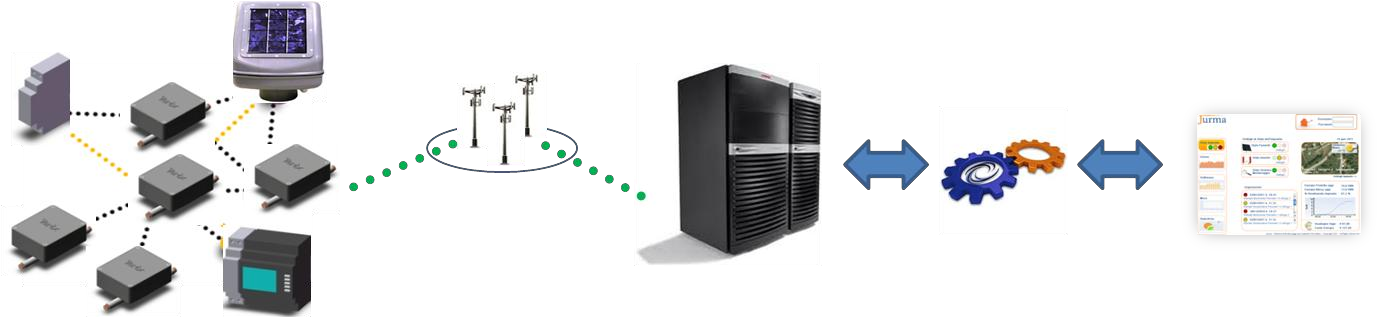
\includegraphics[width=400pt]{img/architecture.png}
\caption{Architettura del sistema}
\label{architettura-sistema}
\end{figure}
%
Nella parte sinistra, \`e presente l'infrastruttura di sensori di campo 
utilizzata per la misura delle grandezze rilevanti.
%
Tale infrastruttura trasmette le letture rilevate mediante una connessione dati 
gprs o gsm ad un \emph{datacenter}, il cui compito \`e quello di processare i dati 
ricevuti, produrre report e allarmi, e pubblicare tutto ci\`o mediante dei 
\emph{web services}.
%
Infine, nella parte pi\`u a destra della figura, \`e rappresentato il \emph{portale web} 
che, utilizzando i servizi web esposti dal datacenter come sorgente dati, fornisce 
una rappresentazione visuale e interattiva dei dati prodotti dal sistema.
%

%
Cominciamo l'analisi del sistema dalla infrastruttura dei sensori di campo.
%
In particolare, in questo capitolo, vedremo quali grandezze si \`e scelto di misurare 
e quali sono state le scelte tecnologiche per la realizzazione della infrastruttura.
%

%
\section{Grandezze rilevanti}
\label{sec:grandezze-rilevanti}
%
La classificazione degli utenti proposta in \cite{kolodenny08} pu\`o essere utile ai 
fini dell'individuazione delle grandezze rilevanti. Le esigenze di monitoraggio 
espresse nell'introduzione a questo capitolo, infatti, prevedono che il sistema 
sia in grado di produrre sia le informazioni cui tipicamente sono interessati i 
\emph{proprietari} degli impianti, sia le informazioni utili ai \emph{manutentori} 
per rilevare malfunzionamenti ed, eventualmente, effettuare diagnosi.
%

%
Alla luce di ci\`o, sono state individuate come rilevanti per un generico impianto 
caratterizzato dalla seguente configurazione,
%
\begin{itemize}
\item $NI$, numero di inverter.
\item $NS_k, k \in \{1, \dots, NI\}$, numero di stringhe dell'inverter $k$.
\item $\eta _{k}, k \in \{1, \dots, NI\}$, rendimento in potenza
  dell'inverter $k$ (rapporto tra
  potenza in uscita e potenza in ingresso).
\item $NP_{j,k}, k \in \{1, \dots, NI\}, j \in \{1, \dots, NS_k\}$, numero
  di pannelli della stringa $j$ legata all'inverter $k$.
\item $\mu _{i,j,k}, k \in \{1, \dots, NI\}, j \in \{1, \dots, NS_k\}, i \in
  \{1, \dots, NP_{j,k}\}$, rendimento in potenza del pannello $i$ della stringa
  $j$ dell'inverter $k$ (rapporto tra  potenza in uscita e irraggiamento).
\item $S _{i,j,k}, k \in \{1, \dots, NI\}, j \in \{1, \dots, NS_k\}, i \in
  \{1, \dots, NP_{j,k}\}, (m^2)$, Superficie del pannello $i$ della stringa
  $j$ dell'inverter $k$.
\end{itemize}
%
le grandezze definite nel seguente \emph{schema}, il quale non si limita ad elencarle, 
ma definisce anche quali grandezze si \`e deciso di misurare direttamente e 
quali, invece, si \`e deciso di stimare:
%
\begin{enumerate}
%%
\item Dati Ambientali:
\begin{itemize}
\item $T, (\deg C)$, Temperatura ambiente.
\item $R, (W/m^2)$, Irraggiamento.
\end{itemize}
%%
%%
\item Grandezze da \textbf{misurare} a monte del contatore bidirezionale:
\begin{itemize}
%%
\item$E_O, (KWh)$, Energia attiva totale prodotta.
\item$P_O, (KW)$, Potenza attiva.
\item$PR_O, (KW)$, Potenza reattiva.
\item$V_O, (V)$, Tensione.
\item$I_O, (A)$, Corrente.
\item$PF_O, (adimensionale)$, Sfsamento (power factor o $cos \phi$).
%%
\end{itemize}
%%
%%
\item Grandezze da \textbf{misurare} a valle dell'inverter $k$:
\begin{itemize}
%%
\item$Iout_{k}, (A)$, Corrente generata.
%%
\end{itemize}
%%
%%
\item Grandezze da \textbf{stimare} per l'inverter $k$:
\begin{itemize}
%%
\item$Vout_{k} = V_O, (V)$, Tensione generata.
\item$Pout_{k} = Vout_{k} \cdot Iout_{k}  \cdot PF_O, (KW)$ Potenza
  (attiva) generata
\item$Pin_{k} = \frac{Pout_k}{\eta _k}, (KW)$, Potenza in ingresso
  all'inverter generata dalle stringhe.
%%
\item$Vin_{k} = \frac{Pin_k}{\sum_{j=1}^{NS_k}{Is_{j, k}}}, (V)$, Tensione
  in ingresso all'inverter
  calcolata sulla base della corrente prodotta dalle stringhe.
%%
\end{itemize}
%%
%%
\item Grandezze da \textbf{misurare} a valle della stringa $j, k$:
\begin{itemize}
%%
\item$Is_{j, k}, (A)$, Corrente generata dalla stringa.
%%
\end{itemize}
%%
%%
\item Grandezze da \textbf{stimare} per la stringa $j, k$:
\begin{itemize}
%%
\item$Vs_{j, k} = Vin_{k}, \forall k, (V)$, Tensione generata da ogni stringa.
\item$Ps_{j, k} = Vs_{j,k} \cdot Is_{j,k}, (KW)$, Potenza generata da ogni
  stringa.
%%
\end{itemize}
\end{enumerate}
%

%
Come vedremo in seguito, tale schema \`e assolutamente \emph{generico}. 
%
La modularit\`a che caratterizza il sistema implementato permette, infatti, 
di scegliere tra due possibili \emph{profili di monitoraggio}: uno \emph{basic}, 
pi\`u economico, che si limita alla sola misurazione della potenza scambiata con 
la rete al fine di monitorare la produzione energetica dell'impianto (tale soluzione 
\`e ideale nel caso di impianti di piccola dimensione) e uno \emph{pro}, che effettua 
la misurazione di tutte le grandezze riportate nello schema (ed \`e pi\`u adatto a 
impianti di grandi dimensioni, dove diagnosticare un malfunzionamento richiede 
una conoscenza di livello pi\`u approfondito dello stato dell'impianto).
%

%
\section{Dispositivi di campo}
Per la misura delle grandezze rilevanti, si \`e deciso di seguire l'approccio
proposto in \cite{xiaoli11}, ovvero l'implementazione di una WSN basata 
su ZigBee. 
%
Questo tipo di soluzione \`e particolarmente adatta alle nostre esigenze, 
in quanto non prevede alcun tipo cablaggio; inoltre, i transponder 
ZigBee sono noti per i loro profili di consumo \emph{ultra-low power}: 
ci\`o permette di alimentare i dispositivi con batterie al litio per un periodo 
di tempo dell'ordine degli anni, e, quindi, permette ai dispositivi di essere
totalmente indipendenti da fonti di alimentazione esterna; per le WSN ZigBee, inoltre, 
esistono dei profili applicativi che prevedono il \emph{set up} automatico, 
ovvero l'autoconfigurazione, della WSN, senza alcuna necessit\`a di intervento 
umano.
%

%
Per effettuare le misurazioni, sono stati previsti due tipi di dispositivi di 
campo: \emph{power/inverter transponders}, e \emph{string transponders}.
%
Un terzo tipo di componente, il \emph{gateway}, funger\`a da \emph{coordinatore}
della WSN e da \emph{concentratore} dati, i.e. interrogher\`a a turno ciascuno
dei nodi della WSN e invier\`a i dati di campo raccolti al datacenter mediante 
gsm o gprs.
%

%
\subsection{Gateway}
%
Come anticipato, il \emph{Gateway} costituisce il \emph{coordinatore} della 
WSN formata dai dispositivi di campo.
%
In quanto tale, si occupa di raccogliere le misure effettuate dai sensori 
e di trasmetterle al datacenter.
%
\begin{figure}[!h]
\centering
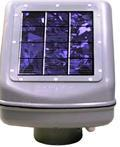
\includegraphics[width=100pt]{img/gw.jpg}
\caption{Gateway}
\label{gw}
\end{figure}
%

%
Come visibile dalle figure \ref{gw} e \ref{gw-opened}, il dispositivo \`e composto 
da un insieme di componenti integrati, che includono, tra gli altri,  \Item{i} il 
modem gsm/gprs, \Item{ii} il transponder radio ZigBee, \Item{iii} la batteria, 
\Item{iv} un fusibile per l'attivazione della rete wireless e \Item{v} un 
piccolo modulo fotovoltaico sulla cover.
%
Tale elemento \`e funzionale sia alla ricarica delle batteria, sia alla stima
del valore di irraggiamento sul campo.
%
\begin{figure}[!h]
\centering
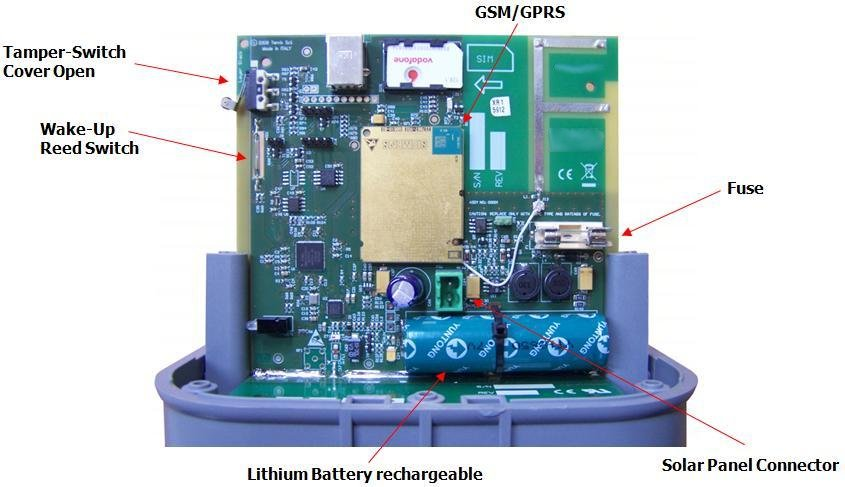
\includegraphics[width=350pt]{img/gw-opened.jpg}
\caption{Elettronica interna del gateway}
\label{gw-opened}
\end{figure}
%

%
Il gateway effettua l'interrogazione dei dispositivi di campo ad intervalli 
predefiniti; la durata dell'intervallo pu\`o essere configurata da remoto, a seconda 
delle esigenze di monitoraggio, i.e. a seconda del rate di campionamento
delle grandezze rilevanti desiderato.
%

%
Una volta raccolte, le misure di campo vengono memorizzate in una memoria locale, 
ed inviate periodicamente al datacenter.
%
La modalit\`a predefinita di trasferimento utilizza una connessione gprs, ed
in particolare, il protocollo FTP, tuttavia, per operare in aree non coperte da 
connettivit\`a gprs, il dispositivo pu\`o essere impostato in modo da trasferire 
i dati tramite via SMS.
%

%
\subsection{Power/Inverter Transponder}
%
Il \emph{Power/Inverter Transponder} \`e un dispositivo costituito da \Item{i} un 
analizzatore di rete e \Item{ii} un transponder ZigBee.
%
Questi dispositivi sono stati pensati per essere collegati alla rete in alternata 
dell'impianto fotovoltaico e, in particolare, per misurare le grandezze rilevanti 
a monte del contatore bidirezionale (power transponder) e a valle degli inverter 
(inverter transponder).
%

%
Il modello di analizzatore di rete scelto \`e il \emph{Socomec Diris A10}
\cite{dirisa10}, in grado di misurare tensione, corrente, potenza, power factor 
e frequenza sia su linee monofase che trifase.
%
\begin{figure}[!h]
\centering
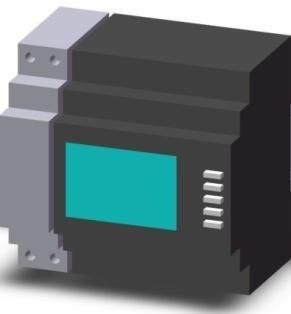
\includegraphics[width=150pt]{img/power-transponder.jpg}
\caption{Socomec Diris A10}
\label{power-transpoder}
\end{figure}
%

%
Gli analizzatori di rete, in genere, non vanno collegati direttamente alle linee di 
potenza su cui effettuare le misurazioni, ma vengono interfacciati mediante dei 
\emph{trasformatori amperometrici} (TA).
%
\begin{figure}[!h]
\centering
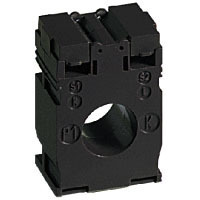
\includegraphics[width=120pt]{img/ta.jpg}
\caption{Trasformatore amperometrico 100/5A}
\label{ta}
\end{figure}
%

%
Essendo dei dispositivi atti alla misura di grandezze di rete in ambito industriale, 
sia gli analizzatori di rete Socomec, sia i TA sono dotati di apposito \emph{attacco} 
per montaggio su barra DIN: ci\`o fa del \emph{quadro di alternata} dell'impianto 
il luogo ideale per l'installazione dei power/inverter transponder.
%

%
\subsection{String Transponder}
%
\begin{figure}[!h]
\centering
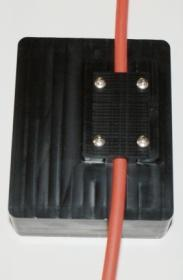
\includegraphics[width=150pt]{img/string-transponder.jpg}
\caption{String Transponder}
\label{string-transponder}
\end{figure}
%
Lo \emph{String Transponder} \`e il dispositivo pensato per la misura delle correnti 
di stringa. \`E anch'esso, come il power/inverter transponder, un dispositivo composito:
\`e costituito da un transponder ZigBee e da un sensore di corrente a \emph{effetto Hall}.
%

%
La scelta dei sensori di corrente induttivi \`e, ancora una volta, frutto della 
necessit\`a di massimizzare la semplicit\`a di installazione del sistema. 
%
Come mostrato in figura \ref{string-transponder}, infatti, l'utilizzo di questi dispositivi
richiede solo che il cavo su cui misurare la corrente venga fatto passare all'interno 
del sensore, senza alcuna necessit\`a di interrompere il cavo stesso.
%

%
\section{Profili di monitoraggio}
Come precedentemente anticipato, sono stati previsti due differenti profili di monitoraggio, 
a seconda del tipo e del numero di transponder che si decide di installare:
%
\begin{itemize}
\item un profilo \emph{basic}, caratterizzato dalla seguente \emph{strumentazione minima}:
      \begin{itemize}
      \item 1 \textbf{Gateway}
      \item 1 \textbf{Power Transponder}
      \end{itemize}
%
\item un profilo \emph{pro}, cui vengono aggiunti, rispetto al profilo \emph{basic} i seguenti 
      moduli \emph{opzionali}:
      \begin{itemize}
      \item n \textbf{Inverter Transponder} (n = numero di inverter)
      \item m \textbf{String Transponder} (m = numero di stringhe)
      \end{itemize}
\end{itemize}
%

%
Il primo profilo, pi\`u economico, \`e stato pensato in maniera specifica per il monitoraggio 
di impianti di piccola taglia. Esso, infatti, monitora esclusivamente l'andamento della produzione
energetica e i dati ambientali.
%

%
Il secondo profilo, invece, si adatta meglio ad impianti grandi e complessi, dove, al fine di 
diagnosticare eventuali cali di rendimento diventa utile monitorare con un livello di dettaglio
maggiore.
% END
 %% architettura del sistema
\clearpage{\pagestyle{empty}\cleardoublepage}
\lstset{language=erlang, basicstyle=\small\ttfamily, keywordstyle=\color{black}, stringstyle=\color{black}, numbers=left, lineskip=0.4\baselineskip, breaklines=true}
\chapter{Il datacenter}\label{sec:datacenter}
%
Il datacenter \`e il componente del sistema responsabile della elaborazione 
del flusso informativo generato dai dispositivi \emph{di campo} installati 
presso i vari impianti sotto monitoraggio.
%
Si tratta di un sistema software costituito da diverse applicazioni, ciascuna 
delle quali implementa una o pi\`u delle funzionalit\`a tra quelle riportate di seguito:
%
\begin{itemize}
  \item decodifica dei \emph{dati di campo}
  \item stima di grandezze \emph{aggregate}
  \item memorizzazione dei dati su \emph{memoria persistente}
  \item rilevamento di \emph{condizioni anomale} e generazione di \emph{allarmi}
  \item fornire accesso allo \emph{stato} degli impianti
  \item fornire accesso ai \emph{dati storici} degli impianti
\end{itemize}
%

%
Dall'elenco delle funzionalit\`a, \`e facile osservare come il
datacenter ricopra un ruolo fondamentale all'interno del sistema di monitoraggio: 
si tratta di un componente \emph{critico}, un suo malfunzionamento 
(ad esempio uno \emph{shutdown} dovuto a un \emph{crash}) puo` avere effetti che 
vanno dalla semplice interruzione del servizio di accesso ai dati degli impianti 
fino alla mancata decodifica dei dati provenienti dai dispositivi di campo e, 
quindi, al blocco \emph{de facto} dell'intero sistema di monitoraggio.
%
Per questo motivo, durante la prima fase della progettazione, sono stati 
individuati, oltre ai gi\`a elencati requisiti funzionali, un insieme di 
\emph{propriet\`a} di cui il datacenter avrebbe dovuto godere. Tali propriet\`a 
sono:
%
\begin{itemize}
\item \emph{liveness}, i.e. una volta verificatosi un evento di interesse, 
il datacenter deve, prima o poi, gestirlo; tale propriet\`a serve a garantire, ad 
esempio, che ogni \emph{batch} di dati provenienti dai dati di campo venga, 
presto o tardi, processato.
%
\item \emph{high availability}, i.e. il datacenter deve essere costantemente 
in esecuzione, salvo \emph{downtime} programmati per operazioni quali 
aggiornamento release, etc.
%
\item \emph{reliability}, i.e. l'esecuzione del datacenter non deve essere 
compromessa da situazioni anomale quali, ad esempio, la ricezione di dati 
\emph{malformati} da parte di dispositivi di campo in avaria. Il datacenter 
deve essere in grado di rilevare potenziali anomalie.%% e segnalarle?
%
\item \emph{scalability}, i.e. le prestazioni del datacenter non devono 
decrescere all'aumentare del numero di impianti, e, quindi del numero di 
flussi informativi, da monitorare. %% e se un giorno volessi distribuire il datacenter?
%
\end{itemize}
%% dire due parole sul fatto che sono proprieta` note?
%

%
Tali propriet\`a hanno fortemente condizionato il successivo \emph{step} di
progettazione, ovvero la scelta della \emph{tecnologia} su cui costruire il 
datacenter, che \`e, infine, ricaduta su Erlang/OTP.
%

%
Il prossimo paragrafo introdurr\`a OTP, soffermandosi su alcuni dei suoi aspetti 
chiave; il paragrafo successivo analizzer\`a le motivazioni che hanno portato alla 
sua scelta quale piattaforma tecnologica; il resto del capitolo, infine, \`e dedicato 
ad alla descrizione dell'architettura e dei componenti del datacanter.
%

%
\section{Breve introduzione a Erlang/OTP}
%
OTP \`e l'acronimo di \emph{Open Telecom Platform}. Rilasciato da \emph{Ericsson} 
a partire dal 1998, si tratta di un \emph{middleware} per applicazioni distribuite 
scritte in Erlang\cite{erlang}. Il suo campo di applicazione, a dispetto di quanto 
il nome possa lasciar intendere, va ben oltre le telecomunicazioni.
%

%
Una definizione pi\`u articolata di cosa sia OTP \`e fornita da Joe Armstrong in 
\cite{armstrong07}: \emph{OTP is an application operating system and a set of libraries 
and procedures used for building large-scale, fault-tolerant, distributed applications}.
%

%
\subsection{Behaviours}
%
L'intera architettura di OTP si basa sul concetto, fondamentale, di \emph{behaviour}:
un behaviour \`e un componente astratto che implementa un determinato 
\emph{design pattern} tipico della \emph{programmazione concorrente}, p.es. il modello di 
interazione \emph{client/server}. 
%
I behaviour OTP, nel loro complesso, forniscono \emph{a set of standardized building 
blocks used in designing and building industrial-grade systems}\cite{cesarini09}.
%
In altre parole, citando \cite{armstrong07}, il loro utilizzo consente agli sviluppatori 
di concentrarsi sulla parte \emph{funzionale} dell'applicazione, i.e. la \emph{business logic}, 
lasciando che il middleware si occupi di gestire gli aspetti \emph{non funzionali}, quali 
\emph{fault-tolerance}, \emph{scalability}, \emph{dynamic code upgrade}, \emph{inter-process 
communication} ecc.
%

%
I behaviour e i moduli application-specific vanno poi collegati, al fine di definire 
un processo Erlang, mediante l'implementazione di opportune \emph{callback}.
%
\begin{figure}[!h]
\centering
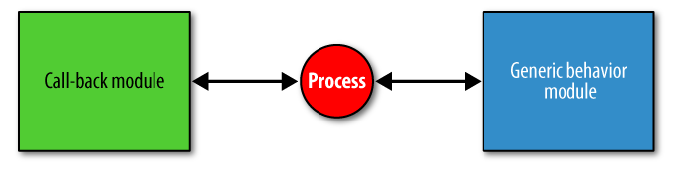
\includegraphics[width=400pt]{img/erl-behaviour.png}
\caption{Processo Erlang costituito da un behaviour e da un modulo di callback}
\end{figure}
%

%
\subsection{Supervision Tree}
%
Esistono due particolari classi di behaviours: \emph{worker} e \emph{supervisor}\cite{otpsupervisor}; 
%
i primi rappresentano i processi che si occupano di effettuare \emph{concretamente} del lavoro, 
p.es. \emph{servers}, \emph{event handlers}, \emph{finite state machines}, ecc.
%
i secondi, invece, si occupano di supervisionare i propri \emph{figli}, i quali possono essere sia
worker che, a loro volta, dei supervisors. 
%
Tra le responsabilit\`a di un supervisor vi sono:
\begin{itemize}
\item \emph{avviare} i processi i figli
\item (opzionalmente) \emph{riavviare} i processi figli in caso di \emph{fault}
\item \emph{terminare} i processi figli al termine dell'applicazione
\end{itemize}
%

%
Il \emph{supervision tree} non \`e altro che una rappresentazione delle relazioni di supervisione 
all'interno di un sistema basato su OTP.
%
\begin{figure}[!h]
\centering
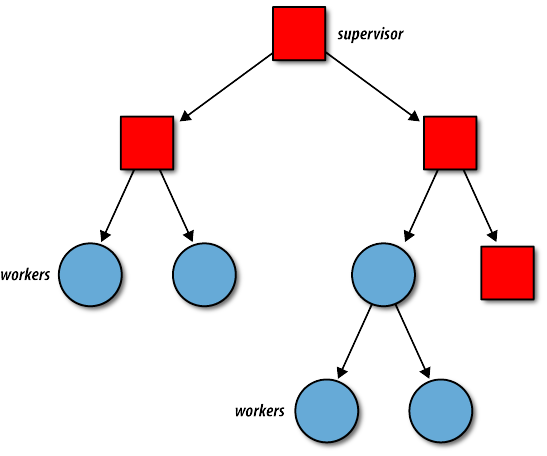
\includegraphics[width=350pt]{img/supervision-tree.png}
\caption{Esempio di supervision tree}
\end{figure}
%

%

%
\subsection{Applications}
%
I supervision tree costituiscono, in un certo senso, lo \emph{scheletro} di ogni applicazione
basata su OTP. Esiste, infatti, un behaviour detto \emph{application}\cite{otpapplication}, 
il cui ruolo \`e quello di raggruppare un insieme di supervision trees, rendendoli 
\emph{riusabili}. 
%

%
In generale, una applicazione OTP \emph{is a reusable component that packages library modules 
together with supervisor and worker processes}\cite{cesarini09}.

%
Una sistema basato su OTP \`e, quindi, formato da un insieme di \emph{application} distribuite 
e \emph{loosely coupled}, ciascuna delle quali implementa una determinata funzionlit\`a.
%

%
\section{Perch\'e OTP}
%
Si \`e scelto di progettare e costruire il datacenter sulla base di Erlang/OTP per i 
seguenti motivi:
%
\begin{itemize}
\item \emph{rapidit\`a di sviluppo}: come gi\`a visto, l'uso dei behaviour consente 
      di concentrarsi sulla business logic di una applicazione; ci\`o \`e particolarmente 
      utile nel caso di applicazioni complesse come il datacenter; 
%% e le caratteristiche 'dichiarative' di Erlang?
%
\item \emph{efficienza e robustezza}: OTP \`e \emph{open source} e, in quanto tale, 
      il suo codice \`e sottoposto a continua revisione e raffinamento; scrivere 
      una applicazione delegando la parte non funzionale a OTP vuol dire, quindi, 
      fare affidamento su una piattaforma assolutamente robusta ed efficiente; 
      a riprova di ci\`o, molti brand famosi utilizzano OTP per alcune delle loro
      soluzioni\cite{whouseserlang}
%
\item \emph{supporto per sistemi sempre online}: i supervisor di un albero possono essere 
      configurati per riavviare i loro worker nel caso in cui questi dovessero, per 
      un qualunque motivo, terminare la loro esecuzione in maniera anormale, i.e. 
      andare in \emph{crash}; ci\`o consente, di fatto, alle applicazioni stesse di
      riavviarsi a seguito di una condizione anomala; OTP elimina persino la necessit\`a
      di mandare offline una applicazione per un \emph{release upgrade}, in quanto 
      supporta l'\emph{hot code swap}
%
\item \emph{rilevamento di crash e recovery}: Erlang pone fortemente l'accento sulla 
      possibilit\`a che i processi possano andare in crash; piuttosto che tentare 
      di prevenire questa eventualit\`a, il linguaggio mette a disposizione gli 
      strumenti necessari per \Item{i} rilevare i crash e \Item{ii} pianificare 
      delle strategie di recupero, e, quindi, per creare sistemi caratterizzati 
      da un elevato grado di \emph{reliability} e \emph{fault tolerance}\cite{armstrongreliability}
%
\item \emph{scalabilit\`a}: uno degli aspetti chiave di Erlang \`e il suo supporto nativo 
      e \emph{sui generis} per la concorrenza; a differenza di altri linguaggi di programmazione, 
      infatti, il modello di concorrenza  implementato da Erlang \`e totalmente indipendente da 
      quello del sottostante sistema operativo, i.e. non esiste un mapping 1-a-1 tra processi 
      Erlang e processi di sistema; ci\`o consente alle applicazioni scritte in Erlang di 
      scalare molto facilmente, come Ghodsi e Armstrong dimostrano in \cite{armstrongyaws}
\end{itemize}
%
%% utilizzo di eunit

%% architettura: insieme di erlang applications:
\section{L'architettura del datacenter}
\label{datacenter-arch}
%
Il datacenter \`e costituito dalle seguenti applicazioni, ciascuna caratterizzata da un 
proprio supervision tree:
%
\begin{itemize}
\item \texttt{database}
\item \texttt{sysconf}
\item \texttt{datamanager}
\end{itemize}
%
Oltre a queste tre applicazioni, il datacenter espone dei web service \emph{RESTful}, 
sfruttando il web server \emph{yaws}\cite{yaws}.
%

%
\section{L'applicazione \emph{database}}
%
Il datacenter si affida a un database MySQL\cite{mysql} per memorizzare in maniera persistente
%
\begin{itemize}
\item la configurazione degli impianti sotto monitoraggio, 
      i.e. quantit\`a, modello e numero di serie dei moduli, numero di stringhe, 
      quantit\`a modello e numero degli inverter, associazioni tra stringa e inverter, ecc.
%
\item le informazioni ricevute dai componenti di campo
\end{itemize}
%
Lo schema relazionale del database \`e mostrato in figura \ref{ermodel}.
%
\begin{figure}[!h]
\centering
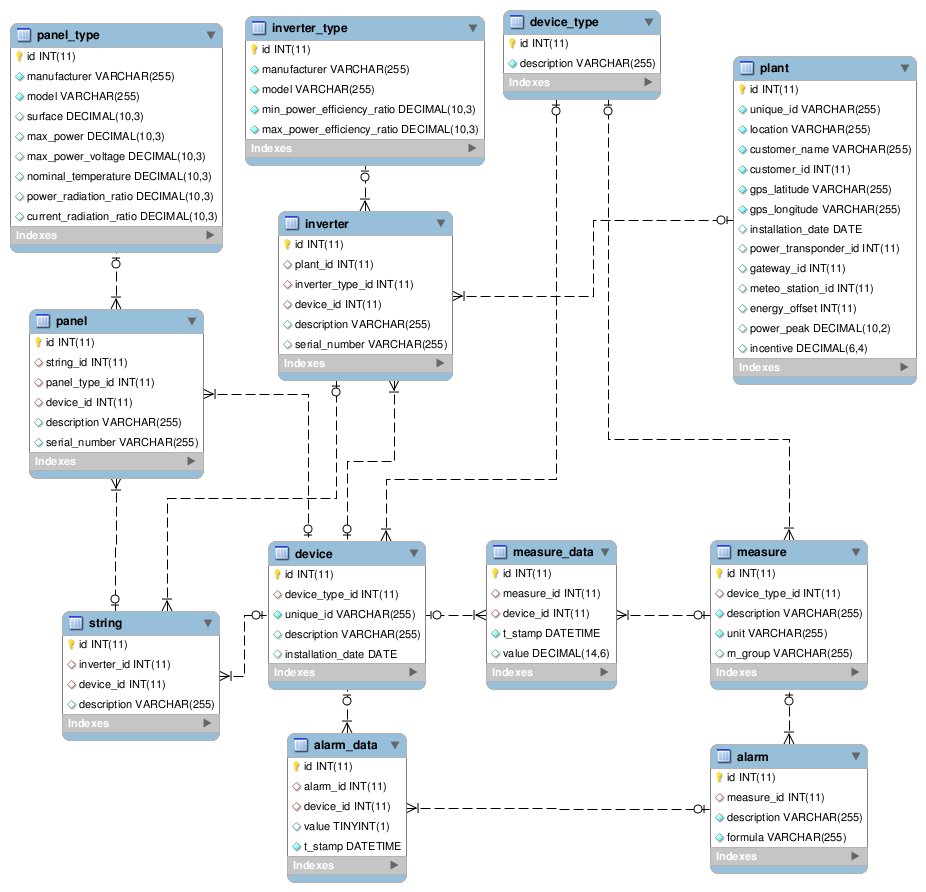
\includegraphics[width=400pt]{img/db-er-model.png}
\caption{Diagramma ER del database}
\label{ermodel}
\end{figure}
%

%
L'applicazione \texttt{database} costituisce, nel contesto del datacenter, 
l'unico punto di accesso alla memoria persistente.
%
Essa \`e interamente basata su \texttt{amnesia}\cite{erl-amnesia}, un wrapper Erlang 
per MySQL, il quale fornisce sia le funzioni per interagire con il database, 
sia gli strumenti necessari a creare dei record erlang per la rappresentazione 
delle entry delle tabelle.
%
In particolare, per le tabelle dello schema relazionale in figura \ref{ermodel}, 
\texttt{amnesia} ha generato i record elencati nel listato \ref{code:database-record}.
%
\begin{lstlisting}[caption={Record per interfacciamento con il database}, label={code:database-record},frame=trBL]
-record (device_type, { ...
-record (device, { ...
-record (measure, { ...
-record (alarm, { ...
-record (inverter_type, { ...
-record (panel_type, { ...
-record (plant, { ...
-record (inverter, { ...
-record (string, { ...
-record (panel, { ...
-record (measure_data, { ...
-record (alarm_data, { ...
\end{lstlisting}
%
Il supervision tree dell'applicazione, mostrato in figura \ref{database-suptree}, \`e molto 
semplice: sono presenti solo \Item{i} un supervisor e \Item{ii} un processo worker, 
\texttt{data\_storage}, il quale implementa il behaviour OTP \emph{gen\_server}\cite{gen-server}.
%

%
\begin{figure}[!h]
\centering
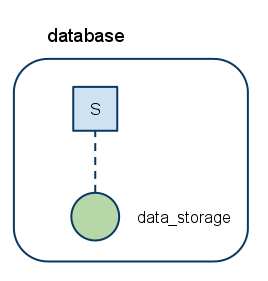
\includegraphics[width=180pt]{img/database.png}
\caption{Supervision tree dell'applicazione Database}
\label{database-suptree}
\end{figure}
%

%
L'interfaccia di \texttt{data\_storage}, le cui funzioni pi\`u importanti sono 
elencate nel listato \ref{code:data_storage_interface}, permettono di:
%
\begin{itemize}
\item aggiungere un impianto
\item modificare la configurazione di un impianto o di uno dei suoi componenti
\item memorizzare i dati di monitoraggio, i.e. il valore delle grandezze monitorate e degli allarmi
\end{itemize}
%

%
\begin{lstlisting}[caption={Interfaccia del modulo \texttt{data\_storage}}, label={code:data_storage_interface},frame=trBL]
-export([%% functions to add new entries
         add_new_device_type/2,
         add_new_inverter_type/3,
         add_new_panel_type/3,
         ...
         add_new_string/2,
         add_new_inverter/2,
         add_new_plant_by_structure/7,
         ...
         set_plant_gateway/4,
         set_string_transponder/6,
         ...    
         %% functions to store monitoring data
         write_variables/1,
         write_alarms/1,
         ...

         %% functions to query the db
         get_plant/1,
         get_plant_structure/1,
         get_plant_devices/1,
         ...
         get_trend_by_device/3
	]).
\end{lstlisting}
%
Il listato \ref{code:new_plant} riporta un esempio di come aggiungere un nuovo impianto
a quelli gi\`a presenti. In particolare, l'esempio mostra come utilizzare la funzione 
\texttt{add\_new\_plant\_by\_structure/7} per aggiungere un impianto costituito da un 
solo inverter a da una sola stringa ad esso connessa.
%
Dopo aver creato il nuovo impianto, mediante la funzione \texttt{set\_plant\_gateway/4}
viene memorizzato sul database anche l'indirizzo fisico del gateway dell'impianto.
%

%
\begin{lstlisting}[caption={Inserimento di un nuovo impianto}, label={code:new_plant},frame=trBL]
%% specify the string configuration
%% i.e., its id and the configuration of each pv module
String = {"String-01", 
          [{"SOVELLO", "SV-X-200", "0000-0000"}]},

%% tell data_storage to create the new plant
data_storage:add_new_plant_by_structure (
      _UniqueID = "MyPlant", 
      _Location = "Nowhere",
      _CustomerName = "Nobody", 
      _Customer_ID = 0,
      _Latitude = "0.0", 
      _Longitude = "0.0",
      %% just one inverter, with the string specified above
      _Inverters = [{{"YURAKU", "I-3000"}, 
                    "Inverter-00", "0000-0000-0000", 
                    [String]} ]),
    
%% set the plant gateway
data_storage:set_plant_gateway (
      _Plant = {unique_id, "MyPlant"}, 
      "E700001A", 
      "", 
      null).
\end{lstlisting}
%

%
\section{L'applicazione \texttt{sysconf}}
%
L'applicazione \texttt{sysconf} fa da supporto all'intero datacenter.
Essa comprende i processi mostrati in figura \ref{sysconfsuptree}.
%
\begin{figure}[!h]
\centering
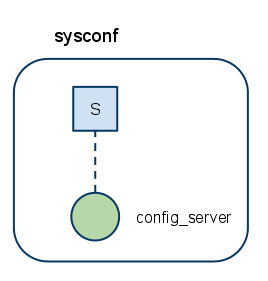
\includegraphics[width=180pt]{img/sysconf.png}
\caption{Supervision tree dell'applicazione Sysconf}
\label{sysconfsuptree}
\end{figure}
%

%
L'unico processo worker presente, \texttt{config\_server}, \`e responsabile della 
gestione e della pubblicazione delle informazioni che costituiscono le configurazioni
dei vari componenti del datacenter. Tali informazioni comprendono,
%
\begin{itemize}
\item le configurazioni dei vari \emph{endpoint} attraverso i quali i gateway possono
      inviare i loro dati al datacenter; p.es. i \emph{path} in cui i \emph{gateway} 
      trasferiscono, via FTP, i file contenenti i dati di campo dei dispositivi;
%
\item le configurazioni dei vari impianti, i.e. quanti e quali dispositivi fanno 
      parte di ogni impianto
\end{itemize}
%
Tali configurazioni sono mantenute nello \emph{stato} del processo: si tratta di un record 
comprendente i seguenti campi:
%
\begin{itemize}
\item \texttt{endpoints\_config}, un record erlang che mantiene le configurazioni dei 
      vari endpoint del sistema
%
\item \texttt{plants}, una tabella che associa, ad ogni impianto, l'elenco dei dispositivi 
      in esso presenti
%
\item \texttt{device\_per\_plant}, una tabella che, dato l'identificatore di un dispositivo,
      permette di risalire all'impianto cui il questo appartiene
\end{itemize}
%

%
La generazione delle configurazioni \`e effettuata durante l'inizializzazione del processo, 
come da listato \ref{code:sysconf-conf-making}.
%
\begin{lstlisting}[caption={Costruzione delle tabelle \texttt{plant} e \texttt{device\_per\_plant}}, label={code:sysconf-conf-making},frame=trBL]
MultiConfigFile = 
  ConfigDir ++ ?MAIN_CONFIGURATION_FILE,

MultiConfigList = 
  conf_manager:load_config(MultiConfigFile),

ParsedConfig = 
  get_configurations(ConfigDir,MultiConfigList),

TableOptions = [set, private, named_table, 
                {read_concurrency, true}],

PlantConfigs = ets:new (plant_configs, TableOptions),
DeviceTable = ets:new (device_table, TableOptions),
    
{ok, Plants} = data_storage:get_plants (),
lists:foreach (
  fun (Plant) ->
      PlantID = Plant#plant.id,
      {ok, Devices} = 
        data_storage:get_plant_devices (PlantID),

      PlantConfig = 
        [I || {#device { unique_id = I}, _, _} <- 
              Devices],

      DeviceEntries = 
        [{I, P} || {#device { unique_id = I}, _, _} <-
                   Devices,
                   P <- [PlantID]],
	      
      ets:insert (PlantConfigs, {PlantID, PlantConfig}),
      ets:insert (DeviceTable, DeviceEntries)
  end, Plants),

State = #config_server_state { config_dir = ConfigDir,
                               config = ParsedConfig,
     		               plants = PlantConfigs,
			       device_per_plant = DeviceTable
			     },
\end{lstlisting}
%

%
Oltre al processo \texttt{config\_server}, il codice della applicazione \texttt{sysconf}
contiene la definizione di un modulo \texttt{logger}, che sfrutta le funzionalit\`a
offerte dalla libreria \emph{log4erl}\cite{log4erl}, al fine di offrire, la possibilit\`a 
di memorizzare su file delle informazioni riguardo il loro stato d'esecuzione.
%

%
\section{L'applicazione \emph{datamanager}}
%
L'applicazione \texttt{datamanager} \`e il componente che si occupa di gestire il flusso 
informativo originato dai gateway degli impianti monitorati, del filtraggio di tali 
flussi informativi, e della memorizzazione dei dati filtrati sul database.
%

%
Rispetto alle altre applicazioni costituenti del datacenter, il \texttt{datamanager} \`e 
caratterizzato da un supervision tree, rappresentato in figura \ref{datamanagersuptree},
pi\`u complesso: esso infatti \`e costituito da un processo \emph{root}, il quale supervisiona
dei \emph{pool}, uno per ogni impianto da monitorare, ciascuno dei quali \`e costituito da un 
supervisor e da due processi worker: un \texttt{filter} e un processo endpoint.
%
Esistono due tipi di endpoint: \texttt{file\_poller} e \texttt{sms\_manager}. Il primo costituisce
l'endpoint di riferimento per i gateway configurati per trasmettere i loro dati mediante 
protocollo FTP, il secondo, invece, per quei gateway che inviano i loro dati mediante \emph{sms}.
%
Si tratta di processi molto simili, motivo per cui, in questa trattazione, daremo spazio solo al
\texttt{file\_poller}.
%

%
\begin{figure}[!h]
\centering
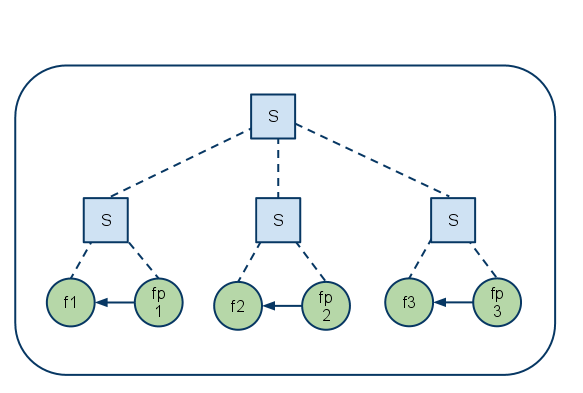
\includegraphics[width=380pt]{img/datamanager.png}
\caption{Supervision tree dell'applicazione Datamanager}
\label{datamanagersuptree}
\end{figure}
%

%
\subsection{Il file\_poller}
%% implementa gen_server
I gateway configurati per l'utilizzo del protocollo FTP inviano al datacenter, 
ad intervalli regolari, un \emph{batch} di file contenenti, ciascuno:
%
\begin{itemize}
\item l'identificatore di un dispositivo di campo
\item un insieme di valori campionati, ciascuno etichettato con un 
      timestamp indicante la data e l'ora del rilevamento
\item informazioni relative allo stato del dispositivo, 
      p.es. lo stato della batteria
\end{itemize}
%
Contestualmente ad ogni \emph{batch}, quale meccanismo di conferma, il gateway invia anche un 
\emph{digest}, riportante l'elenco file inviati.
%

%
Compito del \emph{file\_poller} di un impianto \`e l'effettuazione, ad intervalli di tempo
determinati, delle seguenti operazioni:
%
\begin{enumerate}
\item controlla se il gateway ha trasferito nuovi file; se s\`i,
\item decodifica il digest e leggi l'elenco dei file inviati
\item decodifica il contenuto dei file
\item \emph{passa} le informazioni decodificate al processo \texttt{filter} dell'impianto
\item sposta i file decodificati in un archivio
\item compila dei report riguardo
      \begin{itemize}
      \item eventuali dati non arrivati
      \item eventuali dati \emph{malformati}
      \end{itemize}
\end{enumerate}
%
Questa sequenza di operazioni \`e modellata in figura \ref{fig:polling-sequence} come una
macchina a stati finiti, in cui ogni stato rappresenta una funzione erlang definita nel 
modulo \texttt{file\_poller}.
%
\begin{figure}[!h]
\centering
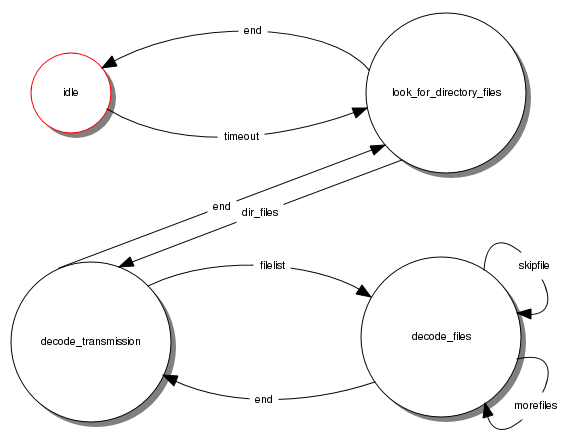
\includegraphics[width=300pt]{img/file-poller.png}
\caption{Sequenza di polling}
\label{fig:polling-sequence}
\end{figure}
%

%
Lo stato \texttt{decode\_files}, all'interno del quale avviene la decodifica dei singoli file,
\`e caratterizzato da due archi \emph{self-connecting}: uno etichettato con \emph{more files}, 
l'altro etichettato con \emph{skip files}.
%
La semantica di queste etichette rispecchia il comportamento della funzione corrispondente 
allo stato \texttt{decode\_files}, riportata nel listato \ref{code:decode_files}. A tale funzione 
va passata la lista dei file da decodificare, lei provveder\`a a decodificarne il primo; quindi, 
se ci saranno ancora \emph{altri file} da decodificare, chiamer\`a se stessa ricorsivamente; 
se la decodifica dovesse fallire (ad esempio perch\`e il formato del file non \`e corretto), 
la funzione \emph{ignorer\`a} quel file e prover\`a a decodificare i rimanenti.
%

%
\begin{lstlisting}[caption={Decodifica dei dati}, label={code:decode_files},frame=trBL]
decode_files ([], Data, State) -> lists:reverse (Data);

decode_files ([File|Rest], Data, State) ->
  Path = State#state.path,
  Result = 
    try
     {ok, FileContent} = 
       file:read_file (lists:concat ([Path, File])),
                       ftp_protocol:decode (FileContent),

     ftp_protocol:decode (FileContent)
		
    catch error : {Reason, D} 
      when (Reason == badmatch) or 
           (Reason == badtimestamp) or
           (Reason == badpreamble) or 
           (Reason == unknown_device_class) -> 
		
      % mark the file as corrupted
      insert_corrupted_file (
        State#state.corrupted_transmissions,
    	{parse_timestamp(File), File}), 
      %% then, return no data
      nil
    end,
    
  case Result of 
    {ok, {DeviceID, DecodedData}} ->
      decode_files (Rest, 
                    [{DeviceID, DecodedData} | Data], 
                    State);
    _->
      decode_files (Rest, Data, State)
  end.
\end{lstlisting}
%

%
Dal listato \ref{code:decode_files} \`e possibile vedere che il \texttt{file\_poller}, rilevato
un file corrotto, invoca la funzione \texttt{insert\_corrupted\_file/2}. Compito di questa funzione 
\`e quello di memorizzare il file corrotto all'interno della \emph{tabella dei file corrotti}, 
i.e. una tabella facente parte dello stato del \texttt{file\_poller}, il cui scopo \`e quello
di tenere traccia dei file corrotti ricevuti.
%

%
Utilizzando lo stesso approccio, il \texttt{file\_poller} tiene anche traccia dei file \emph{missing}, 
i.e. di quei file indicati nei digest inviati dal gateway ma non ricevuti.
%

%
Ad intervalli di tempo determinati, il contenuto delle tabelle viene utilizzato per compilare dei 
\emph{report}, come quello riportato nel listato \ref{code:report-missing-files}, che vengono 
successivamente salvati su file.
%
\begin{lstlisting}[caption={Esempio di report per dati mancanti}, label={code:report-missing-files},frame=trBL]
Received transmission @ {{2011,6,24},{10,18,0}} --> files missing:
    "FFFFFFFF10003000_07DB06180A1200.DAT"
    "FFFFFFFF1000AA00_07DB06180A1200.DAT"
    "FFFFFFFF1000A000_07DB06180A1200.DAT"
    "FFFFFFFF10000300_07DB06180A1200.DAT"
    "FFFFFFFF1000B000_07DB06180A1200.DAT"
    "FFFFFFFF12000500_07DB06180A1200.DAT"
Report generated @ {{2011,6,30},{0,30,40}}
\end{lstlisting}
%

%
Scopo dei report \`e quello di fornire rapidamente delle informazioni precise utili a diagnosticare 
eventuali \emph{fault} di uno qualsiasi dei componenti di campo del sistema di monitoraggio.
%

%
\subsection{La decodifica: \emph{ftp\_protocol}}
%
I file contenenti i dati di monitoraggio inviati dal gateway non hanno tutti lo stesso formato.
%
Esso varia, in generale, a seconda del tipo di dispositivo di campo. Per questo motivo, 
l'operazione di decodifica dei file \`e delegata a un modulo, \texttt{ftp\_protocol}, 
il quale \`e in grado di riconoscere il formato di un file e, quindi, di decodificarlo 
correttamente.
%

%
Le funzioni di decodifica di \texttt{ftp\_protocol} fanno sfruttano la \emph{bit syntax}, una 
sintassi per espressioni Erlang in grado di rappresentare dati binari \emph{raw}.
%
Un esempio d'uso di tali espressioni \`e contenuto nel listato \ref{code:decode-gateway}: si tratta
delle prime righe della funzione \texttt{decode\_gateway\_sample}, il cui compito \`e quello di 
decodificare il singolo campione dati ricevuto da un gateway.
%
\begin{lstlisting}[caption={Decodifica di un blocco dati del Gateway}, label={code:decode-gateway},frame=trBL]
decode_gateway_sample (TemixID, Year, DataBlock, N, Accumulator) ->
    << Battery:2/big-unsigned-integer-unit:8,
       Temperature:2/big-signed-integer-unit:8,
       SolarPanelCurrent:2/big-signed-integer-unit:8,
       Month:8,
       DayOfMonth:8,
       Hour:8,
       Minute:8,
       Rest/binary >> = DataBlock,
       ...
\end{lstlisting}
%

%
\subsection{Il filter}
%% implementa gen_server
Il processo \texttt{filter} si occupa del \emph{filtraggio} dei dati di monitoraggio, i.e.
\begin{itemize}
\item scalare i valori di alcune grandezze, in base alle unit\`a di misura che si desidera
      utilizzare per la loro rappresentazione
%
\item incrementare gli offset delle misure di energia, nel caso venga rilevato un \emph{overflow}
%
\item stimare grandezze \emph{aggregate}
%
\item memorizzare i dati ricevuti sul database
%
\end{itemize}
%
I processi \texttt{filter} lavorano a stretto contatto con gli endpoint di un impianto. 
%
Espongono loro una funzione d'interfaccia, \texttt{put\_variables/4}, mediante la quale 
questi ultimi possono passargli i dati di monitoraggio ricevuti e decodificati.
%

%
Le attivit\`a svolte a \emph{run-time} dal processo \texttt{filter} sono schematizzate in 
figura \ref{filter}: nella parte superiore \`e rappresentata l'attivit\`a di filtraggio 
dei dati di campo; il \emph{triggering event} di questa attivit\`a \`e l'invocazione della 
funzione \texttt{put\_variables/4}.
%
Nella parte inferiore, invece, \`e rappresentata l'attivit\`a di calcolo delle grandezze 
\emph{aggregate}. A differenza della prima, il \emph{triggering event} di questa attivit\`a
\`e sincrono, trattandosi di un evento generato internamente al processo stesso: 
\`e l'azzeramento di un timer locale, configurabile con un parametro \texttt{aggregates\_period}.
%

%
\begin{figure}[!h]
\centering
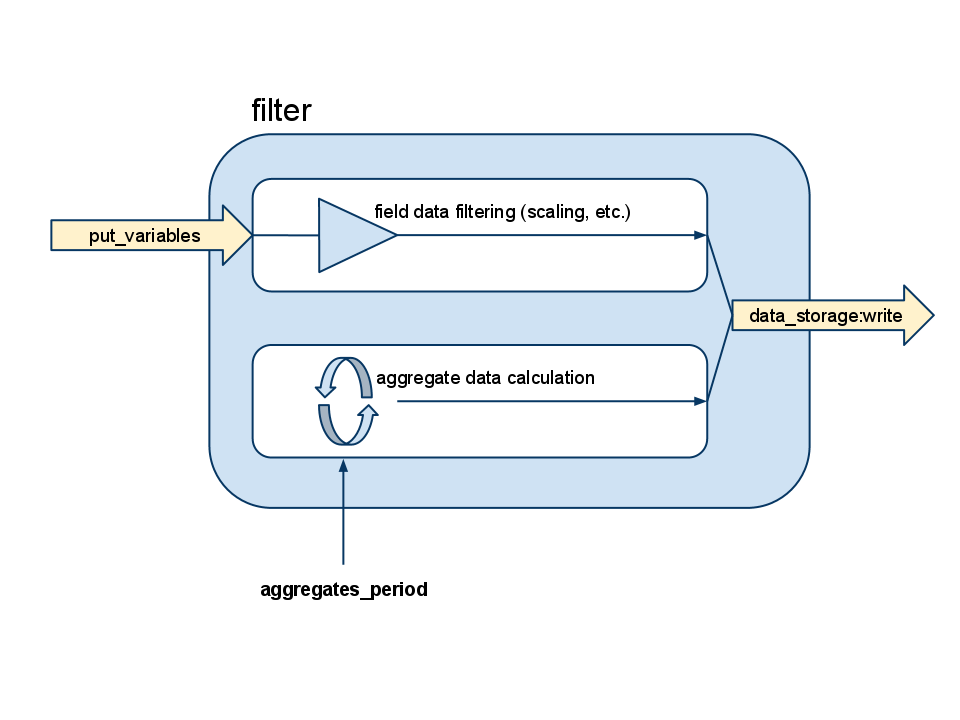
\includegraphics[width=380pt]{img/filter.png}
\caption{Rappresentazione grafica del processo filter}
\label{filter}
\end{figure}
%
Al termine di ciascuna \emph{tranche} di attivit\`a, i dati risultati vengono memorizzati sul 
database, mediante l'invocazione della funzione \texttt{data\_storage:write/4}.
%

\section{Web Services}
%% due parole sui web services restful
 %% il datacenter
%% %\clearpage{\pagestyle{empty}\cleardoublepage}
\chapter{Rappresentazione dei dati}
\label{sec:datapresentation}
%
Una release \emph{preliminare} del sistema di monitoraggio \`e stata installata
presso un impianto fotovoltaico da 100 kWp.
%

%
In particolare, sono stati installati 1 gateway e 1 power transponder.
%
Vengono, di seguito, riportati alcuni dei grafici pi\`u significativi prodotti dal 
\emph{portale web} del sistema di monitoraggio, relativamente a questo impianto.
%
Tutti grafici presentati in questa sezione fanno riferimento allo stesso periodo 
temporale, che va dalle 06:00 alle 20:00 del 23 Giugno 2011.
%

%
In figura \ref{fig:current-power-tr} \`e riportato l'andamento della corrente immessa nella
rete di distribuzione da parte dell'impianto, per ciascuna delle tre fasi. Come \`e possibile
osservare, a meno di piccolissime variazioni, le tre curve coincidono.
%
\begin{figure}[!h]
\centering
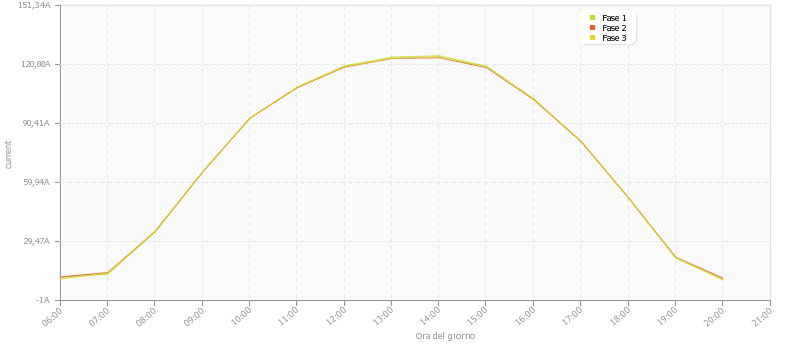
\includegraphics[width=400pt]{img/portale/current-power-transponder.png}
\caption{Corrente immessa in rete}
\label{fig:current-power-tr}
\end{figure}
%
Stesso discorso, ovviamente, vale per la tensione di rete rilevata sulle tre fasi (figura \ref{fig:voltage-power-tr}).
%

%
\begin{figure}[!h]
\centering
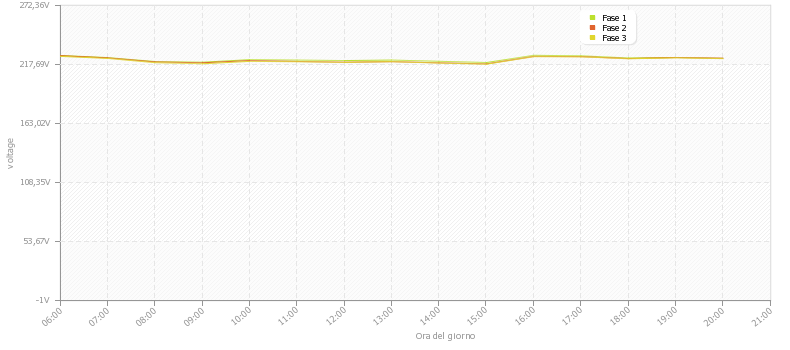
\includegraphics[width=400pt]{img/portale/voltage-power-transponder.png}
\caption{Tensione della rete di distribuzione}
\label{fig:voltage-power-tr}
\end{figure}
%

%
Le figure \ref{fig:active-power-tr} e \ref{fig:reactive-power-tr} mostrano, rispettivamente, 
la \emph{potenza attiva} e la \emph{potenza reattiva} immesse in rete.
%
Il trend della potenza attiva immessa in rete segue, come \`e ovvio che sia, l'andamento della 
corrente visto in precedenza. 
%
La somma delle tre componenti di figura \ref{fig:active-power-tr} restituisce la curva di figura 
\ref{fig:total-active-power-tr}, i.e. la potenza attiva immessa in rete da parte dell'impianto
nell'arco della giornata.
%

%
Il confronto delle curve di corrente e potenza con la curva di irraggiamento, presentata in figura 
\ref{fig:irradiance}, permette di effettuare una prima, grezza, analisi dello stato di salute 
dell'impianto; intuitivamente, infatti, tutte queste curve \emph{devono} presentare lo stesso 
andamento.
%

%
\begin{figure}[!h]
\centering
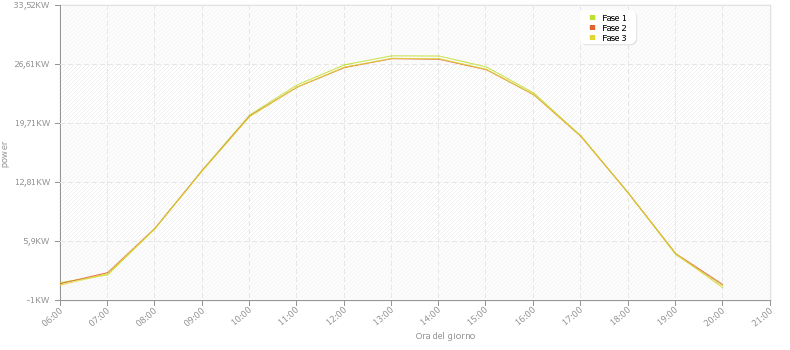
\includegraphics[width=400pt]{img/portale/active-power-transponder.png}
\caption{Potenza attiva immessa in rete}
\label{fig:active-power-tr}
\end{figure}
%

%
\begin{figure}[!h]
\centering
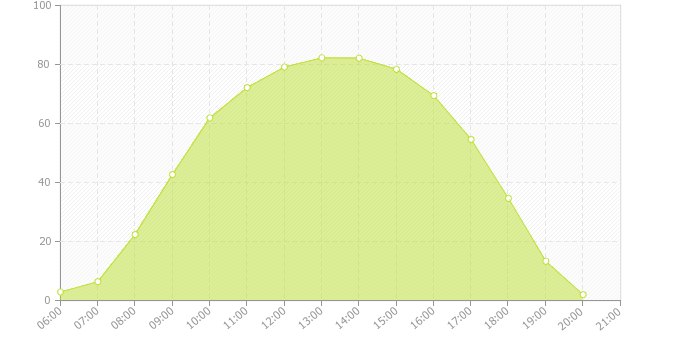
\includegraphics[width=400pt]{img/portale/potenza-giornaliera.png}
\caption{Potenza Attiva - Power Transponder}
\label{fig:total-active-power-tr}
\end{figure}
%

%
\begin{figure}[!h]
\centering
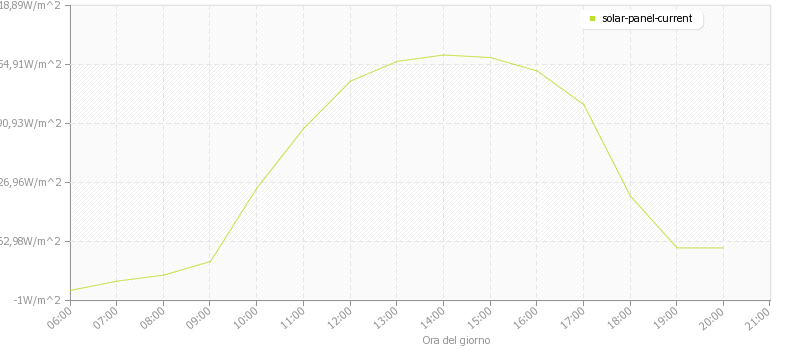
\includegraphics[width=400pt]{img/portale/radiazione-giornaliera.png} %% dire che siamo all'80% del picco
\caption{Curva di irraggiamento}
\label{fig:irradiance}
\end{figure}
%

%
La curva rappresentante il trend della potenza reattiva (figura \ref{fig:reactive-power-tr}), 
invece, permette di verificare, in impianti dotati di sistema di rifasamento, se quest'ultimo
\`e \emph{effective} oppure no. %% e nel nostro caso?
%
\begin{figure}[!h]
\centering
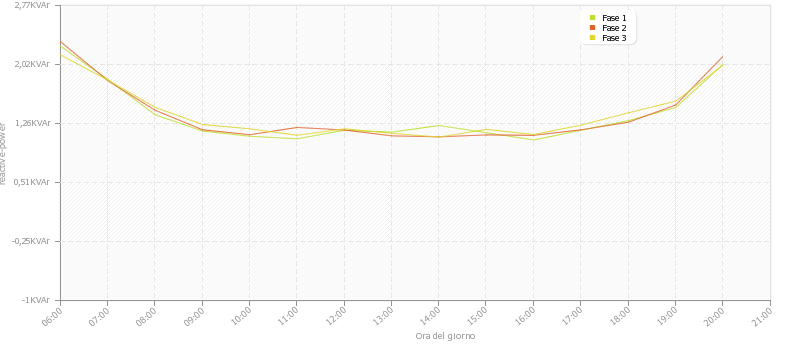
\includegraphics[width=400pt]{img/portale/reactive-power-power-transponder.png}
\caption{Potenza reattiva scambiata con la rete}
\label{fig:reactive-power-tr}
\end{figure}
%
%%Nel caso considerato, il sistema di rifasamento 
 %% caso-studio? qualche esempio di dati prodotti?
\clearpage{\pagestyle{empty}\cleardoublepage}
\chapter{Sviluppi futuri}
blah


%% \appendix
\chapter*{Ringraziamenti}


%% bibliography
\clearpage{\pagestyle{empty}\cleardoublepage}
\begin{thebibliography}{3}
\addcontentsline{toc}{chapter}{Bibliografia}

\bibitem{gse2010} Gestore Servizi Energetici (GSE) \
  - Direzione Studi, Statistiche e Servizi Specialistici, \
  \emph{Rapporto Statistico 2010 -- Solare Fotovoltaico}, 4/2011, 
  http://goo.gl/2DxoQ

\bibitem{photon2010} C. Podewils (2010), \
  \emph{Monitoraggi Immaturi}, \
  Photon - il mensile del fotovoltaico, 8/2010, \
  pagg. 22--24.

\bibitem{bellini09} A. Bellini, S. Bifaretti, V. Iacovone, C. Cornaro, \
  \emph{Simplified model of a photovoltaic module}, \
  Applied Electronics, 2009.                    

%% \bibitem{camera2003} Camera dei Deputati, \
%%   \emph{Decreto Legislativo 29 dicembre 2003, n. 387}, \
%%   http://www.camera.it/parlam/leggi/deleghe/testi/03387dl.htm

%% \bibitem{santoroframe} C. Santoro (2007), \emph{"An Erlang Framework for Autonomous Mobile Robots"}, ACM Erlang Workshop 2007, Freiburg, Germany.

%% \bibitem{siegwart} R. Siegwart, I.R. Nourbakhsh (2004), \emph{Autonomous Mobile Robots}, MIT Press.

%% \bibitem{appinknowledge} Appin Knowledge Solutions (2007), \emph{Robotics}, Infinity Science Press.

%% \bibitem{cohenkoss92} C. Cohen, F. V. Koss (1992), \emph{A Comprehensive Study of Three Object Triangulation}, Mobile Robots VII, SPIE Vol. 1831,1992.

%% \bibitem{beomcho}  Beom H. R., CHO H. S. (1995), \emph{Mobile robot localization using a single rotating sonar and two passive cylindrical beacons}, Robotica vol. 13 (3), pp. 243-252 (15 ref.), Cambridge University Press, 1995.

%% \bibitem{carvalho03} J. S. Esteves, A. Carvalho, C. Couto (2003), \emph{Generalized Geometric Triangulation Algorithm for Mobile Robot Absolute Self-Localization}, International Symposium on Industrial Electronics, Rio de Janeiro, Brazil, June 9-12, 2003.

%% \bibitem {carvalho06} J. S. Esteves, A. Carvalho, C. Couto (2006), \emph{ An improved
%% version of the Generalized Geometric Triangulation algorithm}, II European-Latin-American Workshop on Engineering
%% Systems, Faculdade de Engenharia da Universidade do Porto, Porto, Portugal, June 21-23, 2006.

%% \bibitem {carvalho062} J. S. Esteves, A. Carvalho, C. Couto (2006), \emph{  Position and Orientation Errors in Mobile Robot, Absolute Self-Localization Using an Improved Version of the Generalized Geometric Triangulation Algorithm}, International Conference on Industrial Technology, Mumbai, India, 2006, p. 830-835.

%% \bibitem{whereami} J. Borenstein, H. R. Everett, L. Feng (1996), \emph{"Where am i? Systems and Methods for Mobile Robot Positioning"} \newline http://www-personal.umich.edu/~johannb/shared/pos96rep.pdf 

%% \bibitem{homepage} Eurobot 2008 - DIIT TEAM, \emph{"Eurobot 2008 - DIIT TEAM"} \newline http://eurobot.diit.unict.it/

%% \bibitem{eurobothome} Eurobot Open, \emph{"Eurobot"} \newline http://www.eurobot.org/

%% \bibitem{eurobot2008home} Eurobot 2008, \emph{"Eurobot 2008: Home"}\newline http://eurobot.fh-heidelberg.de/

%% \bibitem{regoleeurobot} Eurobot Open 2008, Mission to Mars \emph{"Rules 2008 - Revision 1"} \newline http://www.eurobot.org/eng/docs/2008/E2008\_Rules-EN-v2.pdf 

%% \bibitem{sitodiit} Eurobot 2008 - DIIT TEAM, \emph{"Docs"} \newline http://eurobot.diit.unict.it/topic-docs.php

%% \bibitem{e3zlr81} Omron Corporation, \emph{"E3Z-LT/LR/LL Data Sheet"} \newline http://www.ia.omron.com/data\_pdf/data\_sheet/e3z-lt\_-lr\_-ll\_dsheet\_csm437.pdf

%% \bibitem{18f2431} Microchip Technology Inc., \emph{"PIC18F2331/2431/4331/4431 Data Sheet"} \newline http://ww1.microchip.com/downloads/en/DeviceDoc/39616C.pdf

%% \bibitem{l293d} STMicroelectronics , \emph{" L293D-L293DD PUSH-PULL FOUR CHANNEL DRIVER WITH DIODES"} \newline http://www.st.com/stonline/products/literature/ds/1330.pdf

%% \bibitem{python} Python Software Foundation , \emph{"Python Programming Language - Official Website"} \newline http://www.python.org/

%% \bibitem{erlang} Erlang, \emph{"Open Source Erlang"} \newline http://www.erlang.org/

%% \bibitem{wikinewton} Wikipedia, \emph{Newton's Method} \newline http://en.wikipedia.org/wiki/Newton\_method

%% \bibitem{wikii2c} Wikipedia, \emph{"I2C"} \newline http://it.wikipedia.org/wiki/I\%C2\%B2C

%% \bibitem{wikilimitecentrale} Wikipedia, \emph{"Teorema del Limite Centrale"} \newline http://it.wikipedia.org/wiki/Teorema\_del\_Limite\_Centrale

%% \bibitem{wikifsm} Wikipedia, \emph{"Finite State Machine"} \newline http://en.wikipedia.org/wiki/Finite\_state\_machine

\end{thebibliography} 


\end{document}
